\documentclass[review]{elsarticle}

\usepackage{multirow}
\usepackage{lineno}
\usepackage{xspace}
%\usepackage{subfig}
\modulolinenumbers[5]

%% Journal name here
\journal{Annals of Nuclear Energy}

%% `Elsevier LaTeX' style
\bibliographystyle{elsarticle-num}
%%%%%%%%%%%%%%%%%%%%%%%

%%%% packages and definitions (optional)
\usepackage{placeins}
\usepackage{booktabs} % nice rules (thick lines) for tables
\usepackage{microtype} % improves typography for PDF
\usepackage{hhline}
\usepackage{amsmath}
\usepackage{graphicx}
\usepackage{subcaption}
\usepackage{pdflscape}

\usepackage{booktabs}
\usepackage{threeparttable, tablefootnote}

\usepackage{tabularx}
\usepackage[table]{xcolor}

%% Special typesetting for Cyclus
\newcommand{\Cyclus}{\textsc{Cyclus}\xspace}%
\newcommand{\Cycamore}{\textsc{Cycamore}\xspace}%
\graphicspath{{images/}}

% tikz %
\usepackage{tikz}
\usetikzlibrary{positioning, arrows, decorations, shapes}

\usetikzlibrary{shapes.geometric,arrows}
\tikzstyle{process} = [rectangle, rounded corners, minimum width=3cm, minimum
height=1cm,text centered, draw=black, fill=blue!30]
\tikzstyle{object} = [ellipse, rounded corners, minimum width=3cm, minimum
height=1cm,text centered, draw=black, fill=green!30]
\tikzstyle{arrow} = [thick,->,>=stealth]

% hyperref %
\usepackage[hidelinks]{hyperref}
% after hyperref %
\usepackage{cleveref}
\usepackage{datatool}
\usepackage[acronym,toc]{glossaries}
%\newacronym{<++>}{<++>}{<++>}
\newacronym{AB}{AB}{AdaBoost}
\newacronym{AI}{AI}{Artificial Intelligence}
\newacronym{ANN}{ANN}{Artificial Neural Network}
\newacronym{AP}{AP}{average precision}
\newacronym{B}{B}{Bagging}
\newacronym{BNB}{BNB}{BernoulliNB}
\newacronym{DT}{DT}{DecisionTree}
\newacronym{EALF}{EALF}{energy corresponding to average lethargy of neutrons causing fission}
\newacronym{EN}{EN}{ElasticNet}
\newacronym{ET}{ET}{ExtraTrees}
\newacronym{EVR}{EVR}{explained variance regression score}
\newacronym{GA}{GA}{Genetic Algorithm}
\newacronym{GB}{GB}{GradientBoosting}
\newacronym{GNB}{GNB}{GaussianNB}
\newacronym{HALEU}{HALEU}{High Assay Low Enriched Uranium}
\newacronym{HL}{HL}{average Hamming loss}
\newacronym{KN}{KN}{KNeighbors}
\newacronym{L}{L}{Lasso}
\newacronym{LL}{LL}{LassoLars}
\newacronym{Log}{Log}{Logistic}
\newacronym{LP}{LP}{LabelPropagation}
\newacronym{LRAPS}{LRAPS}{ranking-based average precision}
\newacronym{LRL}{LRL}{label ranking loss}
\newacronym{MAE}{MAE}{mean absolute error}
\newacronym{ML}{ML}{Machine Learning}
\newacronym{MLP}{MLP}{MultiLayerPerceptron}
\newacronym{MOGA}{MOGA}{Multi-Objective Genetic Algorithm}
\newacronym{MSE}{MSE}{mean square error}
\newacronym{MSR}{MSR}{Molten Salt Reactor}
\newacronym{MSRE}{MSRE}{Molten Salt Reactor Experiment}
\newacronym{NN}{NN}Neural Network}
\newacronym{NSGAIII}{NSGAIII}{non-dominated sorting genetic algorithm}
\newacronym{ORNL}{ORNL}{Oak Ridge National Laboratory}
\newacronym{P}{P}{Perceptron}
\newacronym{PM}{PM}{polynomial mutation}
\newacronym{R}{R}{Ridge}
\newacronym{RF}{RF}{RandomForest}
\newacronym{ROC_AUC}{MAE}{compute area under the receiver operating characteristic curve}
\newacronym{SBX}{SBX}{simulated binary crossover}
\newacronym{SGD}{SGD}{StochasticGradientDescent}
\newacronym{SV}{SV}{SupportVector}
\newacronym{SVM}{SVM}{support vector machine}
\newacronym{UNF}{UNF}{Used Nuclear Fuel}


\makeglossaries


\begin{document}
	
\begin{frontmatter} 
	\title{Machine Learning Application to Single Channel
		Design of Molten Salt Reactor} 
	\end{frontmatter} 
\section*{Highlights}
\begin{itemize} 
\item We proposed a machine learning-enabled optimization approach and validated
in a single channel design of molten salt reactor.
\item Reactor database was generated by the grid sampling strategy for training
dataset and Monte Carlo technique for testing dataset.
\item With extra-trees estimator, performance metrics were successfully
predicted and classified within the 5\% relative error.
\item We determined one optimal design for each fuel-salt couple. 
\item This method accurately predicted performance metrics with no neutron 
transport calculation.
\end{itemize}


	\begin{frontmatter}
		\title{Machine Learning Application to
			Single Channel Design of Molten Salt Reactor}
		
		% Authors
		\author[uiuc]{Mehmet Turkmen\corref{corrauthor}}
\cortext[corrauthor]{Corresponding Author}
\ead{mturkmen@illinois.edu}
\author[uiuc]{Kathryn D. Huff}


		
		% Institutes of the authors
		\address[uiuc]{Dept. of Nuclear, Plasma, and Radiological Engineering,
University of Illinois at Urbana-Champaign, Urbana, IL 61801}

		
		\begin{keyword}
			channel design \sep
			molten salt reactor \sep
			machine learning \sep
			optimization \sep 
			simulation \sep
			Monte Carlo 
		\end{keyword}
		
		\begin{abstract} 

This study proposes an efficient, accelerated and robust approach to design a
nuclear reactor core from scratch, using state-of-the-art machine learning
\gls{ML} techniques. We implemented the recommended approach into a single fuel
channel of a molten salt reactor (MSR) to demonstrate the applicability of the
method. We prepared a Python tool, named Plankton, which couples to a reactor
physics code and the Multi-Objective Genetic Algorithm, and imports \gls{ML}
methods. It performs three consecutive phases: (i) reactor database generation,
(ii) machine learning application, (iii) design optimization. With the
extra-trees method, we found nine optimum designs for each fuel-salt pair and
estimated all the performance metrics of the optimum designs within a prediction
error of $<$5\% with respect to their actual values. U-Pu fuel mixed with NaCl
salt as well as LiF-BeF$_2$ salt gave the promising results, yielding the
highest conversion ratio, the most negative feedback coefficient, and the lowest
fast flux.

\end{abstract}

	\end{frontmatter}
	\glsresetall
	
	%% Shows line numbers
	\linenumbers
	
	\section{Introduction}

    Current applications of learning-based techniques in nuclear engineering indicate that \gls{AI} will soon undertake the role of reactor designers in optimizing the designs of current and future reactors. \gls{AI} methods, more specifically \gls{ML}, have already become important to most sub-fields of nuclear science and engineering (e.g., in-core fuel management, reactor safety, flow regime prediction, and radiation protection) to achieve an optimal core loading map, to make nuclear reactors safer, to quickly comprehend flow data, and to accurately identify critical isotopes in nuclear materials. In this context, recently published two review papers \cite{Gomez2020, Nissan2019} showed the potential, competence, and importance of these methods by exploring the recent studies on the use of learning-based methods in nuclear science and relevant fields. The articles also probed the suitability of the commonly used algorithms and algorithm selection criteria. However, \gls{AI}/\gls{ML} has not contemplated as an option to seek to find optimal designs of nuclear reactor cores despite being a proven technique for optimization. Instead, iterative approaches such as individual parameter searches and evolutionary algorithms have been widely employed for reactor core design optimization.

    Among parametric studies recently reported, Wei \emph{et al.} \cite{Wei2018} investigated several critical feature parameters of a \gls{MSR} channel by parameter interpolation using KENO-VI in SCALE 6.1 \cite{scale2020}. In the study, critical feature parameters are the fuel type, $^{6}$Li concentration, composition of fuel type, channel geometry, moderator and its density, and salt operation temperature. The research showed that $^{6}$Li has a strong effect on criticality. In all different shapes of fuel channels, Wei \emph{et al.} \cite{Wei2018} observed that the turning point from under-moderation to over-moderation for the multiplication factor ($k$) is at a pitch to channel ratio ($P/D$) between 2 and 4, and a fuel volume fraction between 0 and 0.1. Increasing the amount of moderator resulted in an increase in $k$, but then further increase caused a decrease. Meanwhile, the temperature coefficient changes from negative to positive for pitch $>$ 12 cm.

    Anderson \emph{et al.} \cite{Anderson2019} assessed the importance of several parameters (fissile enrichment, lattice pitch, salt-moderator ratio, and the number of fuel channels) in a \gls{MSR} core by looking into the change of fission and removal transition matrices. In that work, the results showed that some of these parameters have an increasing impact on the average relative difference of transition matrices while others have a decreasing effect.

    The common deficiency of both studies is the neglect of strong interdependence of those investigated parameters, by carrying out only a single parametric study. The effect of a single parameter on performance metrics (multiplication factor, conversion ratio, reactivity feedback coefficient, etc.) can be either beneficial or detrimental. As for more than one parameter, correlations between parameters can be seen as superpositioning, canceling out another, or acting on each other up to some extent. Correspondingly, such multi-parameter optimizations would require more sophisticated searching techniques like genetic algorithm, particle swarm, and simulated annealing methods. Unlike parametric studies, these sophisticated optimization techniques are very useful in finding optimal parameters, particularly for multi-objective problems, and are a common and effective way of determining optimal core loading maps \cite{Nissan2019}.

    In the case of using evolutionary algorithms in core designs, Kumar and Tsvetkov \cite{Kumar2015} used a \gls{GA} method coupled to regression splines to optimize several performance metrics such as multiplication factor, fast fission factor, thermal efficiency, and burn up in the design of Gas Cooled Fast Breeder reactor. That method interpolates intermediate values of parameters and metrics. Regarding a fuel pin cell, optimal design values of radius, enrichment fraction, mass flow rate, and coolant temperature at the inlet were found to be 0.22 cm, 18.5 wt. \%, 63.5  $^o$C, and 35.9 kg/s, respectively. Zeng \emph{et al.} \cite{Zeng2020} performed a multi-objective optimization to the Advanced Burner Test Reactor (ABTR) core, a sodium-cooled fast test reactor (SFR), to get an ultimate core design. In that work, an integrated version of the US Department of Energy's Nuclear Energy Advanced Modeling and Simulation (NEAMS) Workbench \cite{neams2019} along with \gls{GA} was used for core modeling and optimization. Although they found about 3150 optimal core designs within Pareto front solutions by optimizing reactivity swing, Pu mass feed, core volume, core power, and peak fast flux, only six candidate designs passed their performance criteria based on their defined constraints.

    Two other important studies \cite{pereira1999, pereira2003} investigated a hypothetical reactor design in a cylindrical fuel rod geometry (i.e., composed of a moderator, clad, and fuel regions) to validate the \gls{GA} applicability and to make a comparison with classical linear optimization methods. In the first study, only two continuous feature parameters were considered for optimization. Optimal designs were completed using 3500 reactor simulations (100 populations and 35 generations). Later, a more complex version of the previous problem was repeated with continuous and discrete variables, very identical to our problem from the aspects of types and number of feature parameters. Optimization results were obtained with 150000 reactor simulations (300 populations and 500 generations).

    Recently published studies \cite{Kim2018, Kim2020} reported the results of an assembly and core design at the Kyoto University Critical Assembly through an \gls{ANN} coupled to MCNP6 \cite{mcnp2017}. These studies are similar to fuel loading pattern optimization studies in terms of the optimization approach. In these works, different core materials, the number of fuel regions, and fuel assembly types were defined as vital feature parameters whereas fast flux and multiplication factor were the target metrics to be optimized.

    Regarding the use of \gls{ML} methods in depletion prediction of reactor applications, Bae \emph{et al.} \cite{Bae2020} successfully predicted Pressurized Water Reactor (PWR) \gls{UNF} composition by training the dense neural network in the Keras \cite{keras2015}. They showed that their proposed model outperforms the average recipe method, one of the transmutation methods which supplies neutronic calculations externally to the nuclear fuel cycle simulators, by yielding less than 1\% error for the \gls{UNF} inventory decay heat and activity and less than 5\% error for the important isotopes.

    As discussed previously, parametric studies which handle all feature variables independently ignore the complex interdependence of these variables and evaluate performance metrics by changing only one feature variable at a time, thus fixing others. Meanwhile, evolutionary algorithms suffer from the choices of optimizer hyperparameters such as population size, number of generations, and cross-over rate since it is unlikely to determine exactly what these parameters would be without making a preliminary calculation. Additionally, these optimization techniques do not provide any flexibility to the designers, such as making optimization without running reactor simulator again when constraints are changed. This hence results in excessive usage of computational resources. Furthermore, optimization methods occasionally converge to local instead of global optima fail to achieve ideal designs that are eliminated by the optimizer's elimination and/or selection criteria. At this point, if sufficient data is supplied, the use of learning-based methods seems rational to design a nuclear reactor because of their exceptional ability to accurately predict performance metrics and appropriate to use with optimization tools as a reactor simulator.

    The \gls{ML} methods, which have not been considered for the sole design of a reactor core so far, will be the best option in this regard. This article compares various \gls{ML} methods in terms of performance scores and recommends employing these methods in place of neutron transport codes for the prediction of performance metrics. This research demonstrates that the proposed method predicts performance metrics more accurately and quickly than the existing optimization techniques.

	\section{Methodology}

In this section, we described how to apply the \gls{ML} methods to design a
reactor core. We followed a methodology consisting of three separate phases: (1)
database generation, (2) machine learning, and (3) design optimization. For
this, we developed a Python tool, called Plankton. The Plankton produces
training and testing datasets for given feature parameters, determines a
\gls{ML} method based on performance scores, trains a predictive model for the
selected \gls{ML} method, predicts performance metrics of designs and finds
optimal designs. The tool calls a reactor physics code to compute the
performance metrics, applies an optimization technique to reveal the optimum
designs and, uses utilities from the scikit-learn tool for the
regression/classification analyses, the quantification of the quality of
predictions, preprocessing and postprocessing. A computational flow chart
showing the main computing steps of the Plankton code is displayed in
Figure~\ref{fig:flowchart}, and the computational steps are detailed in the
following sections.

\begin{figure}[ht!]
	\centering
	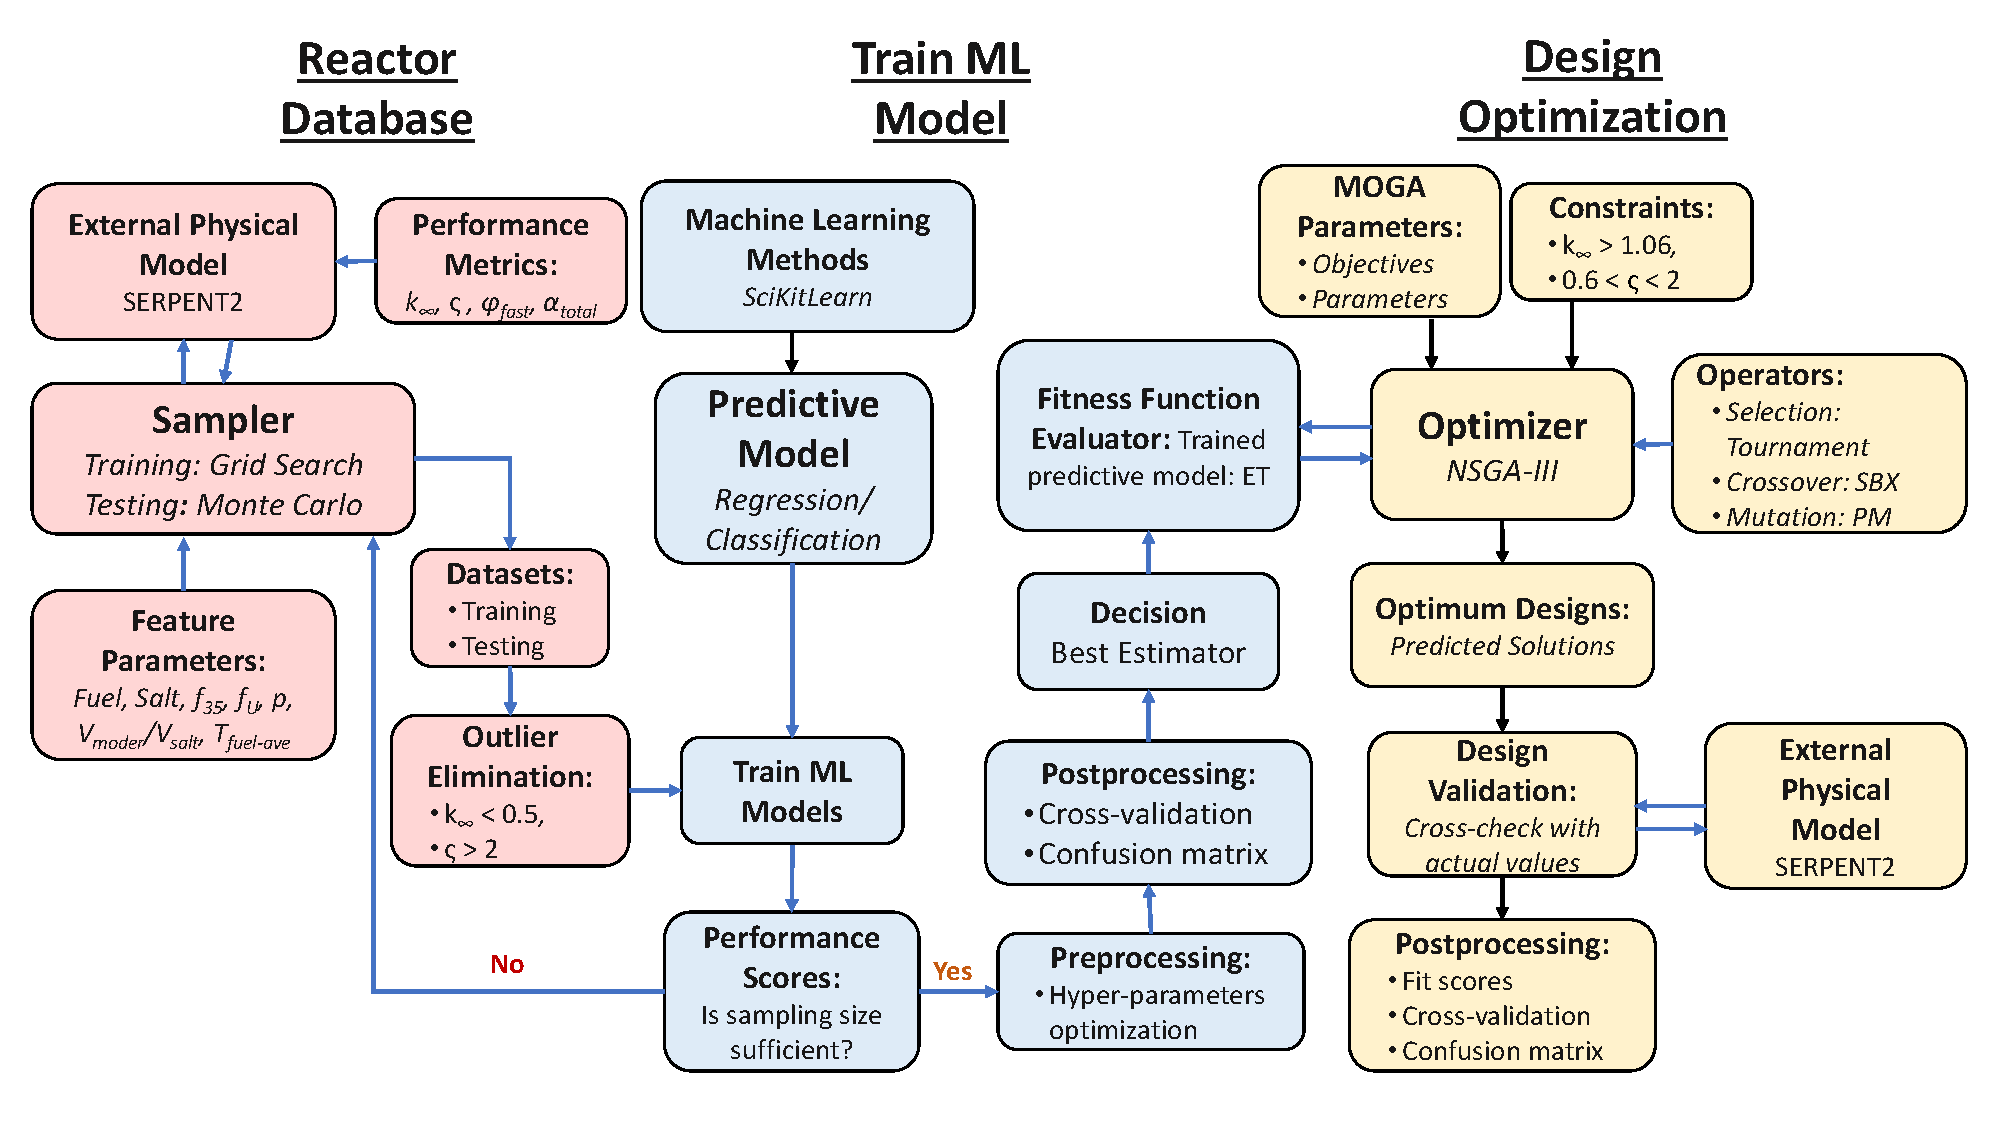
\includegraphics[trim = 0 20 0 20, clip,
	width=\textwidth]{images/computational_flowchart.pdf}
	\caption{Computational flowchart of the Plankton code}
	\label{fig:flowchart}
\end{figure}

 

\subsection{Plankton}

\subsubsection{Database Generation}

The database generation is the step in which samplings in datasets are created
and, training and testing datasets are produced based on two distinctive
sampling strategy, Grid sampling and Monte Carlo.

The grid sampling strategy, the simplest exploration approach to explore an
uncertain domain, was used to obtain the training dataset. It constructs an
N-dimensional grid in which each dimension accounts for a single feature
parameter. A sample in the dataset represents a specific node in the grid.

In contrast to the grid strategy, a test dataset was generated by the Monte
Carlo technique in which the value of each variable is randomly determined
between the lower and upper limits. As the size of samplings has a significant
effect on fitting scores of the training data, the determination criteria for
the size of datasets were explicitly defined in the learning curve section.
Therefore, the estimation of the optimum training sample size is performed by
the 'learning$\_$curve' tool in conjunction with 'ShuffleSplit', which examines
the change in the validation and training score of an estimator for which the
number of training samples varies.

Computational steps performed in database generation phase:
\begin{itemize}
	\item Initialize the feature parameters, properties of which are given in
	Table~\ref{table:features}, for the grid search technique and Monte Carlo
	method.
	\item Prepare the input files for the reactor physics code for neutron
	transport calculation and simulate each sample in training and testing datasets.
	\item Calculate the performance metrics and extract them from the code output.
	\item Supply the prepared reactor database, a set of training/testing samples
	which comprise the feature parameters with corresponding performance metrics, to
	the machine learning phase.
\end{itemize}

\subsubsection{Machine Learning}

In this part, we scoped out various regressors and classifiers from \gls{ML}
methods with the scikit-learn python package \cite{Ped2011}.
Table~\ref{table:AImethods} lists \gls{ML} methods including semi-supervised and
supervised methods such as \gls{NN}, ensemble, linear, \gls{SVM}, decision tree,
naive bayes, and neighbor-based methods. Because there is more than one
performance metric, the estimators need a built-in or external
multi-class/multi-label support. We therefore used the multi-target multi-output
method in regression and multi-label multi-output method in classification when
necessary. In this context, either 'MultiOutput' or 'OneVsRest' tools (e.g., for
\gls{SV} classifier) were utilized. We performed a comprehensive performance
assessment by examining various regression and classification metrics given in
Table~\ref{table:MLmetrics}. Prior to regression/classification analyses, we
standardized our datasets by the MinMaxScaler scaler that scales each feature
parameter between zero and one.

For the optimization of the hyper-parameters of the estimators, we performed an
exhaustive search over specified parameter values using GridSearchCV within the
scikit-learn module to further improve the scores of estimators.

Computational steps performed in machine learning phase:
\begin{itemize}
	\item As a starting point, use diverse \gls{ML} methods, listed in
	Table~\ref{table:AImethods}, from the scikit-learn tool.
	\item With the default settings of hyper-parameters, assess the potential
	estimators to be used in training just by looking into their fit performances
	and exclude the worst ones from the list of the potential estimators.
	\item Analyze the learning curves of the selected estimators to understand
	the optimal sample size required for a high-quality training.
	\item Make a hyper-parameter optimization for the selected estimators to
	further improve the estimators' scores.
	\item Eliminate the outliers for which the performance metrics which seem
	impracticable from the viewpoint of designing a reactor and are out of interest,
	to further improve the estimators' scores, focusing on only the feasible
	solution domain.
	\item Select the best estimator(s) according to their fitting scores.
	\item For better understanding of the selected estimators' capability, get
	the final scores of the estimators, cross-validate the results of the
	regressors, and draw confusion matrices of the classifiers.
	\item Supply the best estimator(s) (along with the optimized
	hyper-parameters) to the design optimization phase to predict the performance
	metrics of the objective functions. 
\end{itemize}

%%%%%%%%%%%%%%%%%%%%%%%%%%%%%%%%%%%%%%%%
\begin{table}[ht!]
	\centering
	\caption{Examined \gls{ML} methods \cite{Ped2011}} 
	\begin{tabular}{ll}
		\hline
		\textbf{Method} & \textbf{Estimator}    \\ \hline
		Ensemble  & \gls{RF}, Bagging (B)  \\
		& AdaBoost (AB), \gls{ET} \\
		& GradientBoosting (GB)   \\
		Linear    & ElasticNet (EN), Perceptron (P), Ridge (R) \\
		& StochasticGradientDescent (SGD)  \\
		& Lasso (L), LassoLars (LL), Logistic (Log) \\
		Naive Bayes     & GaussianNB (GNB), BernoulliNB (BNB)\\
		Neighbor-Based  & \gls{KN} \\
		\gls{SVM} & \gls{SV} \\
		\gls{NN}  & \gls{MLP} \\
		\gls{DT}  & \gls{DT}  \\
		Semi-Supervised & LabelPropagation (LP) \\ \hline
	\end{tabular}
	\label{table:AImethods}
\end{table}
%%%%%%%%%%%%%%%%%%%%%%%%%%%%%%%%%%%%%%%%
\begin{table}[ht!]
	\centering
	\caption{Metrics for performance assessment of estimators \cite{Ped2011}} 
	\resizebox{\textwidth}{!}{%
		\begin{tabular}{ll}
			\hline
			\textbf{Regression}                  & \textbf{Classification}                  \\ \hline
			fit score (fit$\_$score)             & fit score (fit$\_$score)                 \\
			mean square error (MSE)              & average precision (AP)                   \\
			mean absolute error (MAE)            & ranking-based average precision (LRAPS)  \\
			explained variance regression (EVR)  & label ranking loss (LRL)                 \\
			coefficient of determination (R$^2$) & average Hamming loss (HL)                \\
			& computed area under the receiver         \\
			& operating characteristic curve (ROC-AUC) \\ \hline
	\end{tabular}}
	\label{table:MLmetrics}
\end{table}
%%%%%%%%%%%%%%%%%%%%%%%%%%%%%%%%%%%%%%%%

\subsubsection{Design Optimization}

In the final stage of the channel design, we aimed at finding the optimal
designs. We implemented a multi-variable multi-objective evolutionary algorithm.
We selected this method because optimization methods such as gradient-based or
non-linear least-square do not accept discrete and non-numeric variables. We
opted for an optimization method appropriate to the problem's behavior which
manifests a convex structure rather than a linear relationship.

We defined the number of generations as a convergence stopping criterion. After
finding the optimum designs with Plankton's ML methods, we rerun Serpent tool
with the optimal design feature parameters to crosscheck the solutions. Thus, we
performed additional neutron transport calculations for the optimal designs via
the reactor physics code, used to generate the reactor database. Acceptance
criteria for the accuracy of the optimal designs was selected as:
\begin{eqnarray}\label{Eq0}
\dfrac{x_{i,a}-x_{i,p}}{x_{i,a}} \leq 5%
\end{eqnarray}
where $x_{i,a}$ is the actual value of i$th$ metric and $x_{i,p}$ is the predicted 
value of i$th$ metric.

Computational steps performed in design optimization phase:
\begin{itemize}
	\item Initialize the \gls{MOGA} parameters including decision variables,
	operators, number of generations, initial population size, crossover rate
	and mutation ratio.
	\item Define the constraints for the performance metrics which would
	eliminate undesired designs.
	\item Use a \gls{GA} method, which are naturally
	limited by the problem, consistent with the structure of the feature parameters.
	\item Couple the estimator(s) to the \gls{GA} method to calculate the
	performance metrics of the objective functions, without running a reactor physics
	code.
	\item Iterate this \gls{ML}-\gls{GA} coupled system until either the
	constraints are met or the solutions are converged to one of the predefined
	criteria. 
	\item Verify the pareto-front (predicted) solutions by calculating actual
	values.
\end{itemize}

\subsection{Channel Design with Plankton}

\subsubsection{Design Parameters}

We applied the suggested method to a single fuel channel \gls{MSR} geometry with
square unit cell approximation to use in a basic geometry with the least number
of feature parameters and performance metrics. An illustration of the channel
geometry is shown in Figure~\ref{fig:channel}. Feature parameters describing the
material and geometry properties of the single channel were selected as fuel
type, salt type, $^{235}$U fraction ($f_{35}$) in U, U fraction ($f_{U}$) in
heavy metal, channel-to-channel pitch length ($p$), moderator-to-salt volume
ratio ($\xi$), and average fuel-salt temperature ($T_{ave}$) along the channel.
We varied the variables between upper and lower bounds described in
Table~\ref{table:features}. The $^{235}$U fraction in U was limited to 20 wt.\%
which is the maximum limit for \gls{HALEU}. For the fuel types other than U fuel
type, U content in heavy metal varies from 10 to 90 wt.\%. The maximum $p$,
based on \gls{ORNL}'s \gls{MSRE} design, was set to 16 cm. The $\xi$ variable
was calculated from the ratio of pitch to fuel salt radius between 0.274
(p/D$_{fuel}$ = 1) and 10.46 (p/D$_{fuel}$ = 3).

We studied three different fuel types, U, U-Th and U-Pu in this work. Th in U-Th
contains only $^{232}$Th isotope whereas Pu in U-Pu comes from the weapon-grade
Pu constituting the following isotopes: $^{238}$Pu (0.05 at.\%), $^{239}$Pu
(94.3 at.\%), $^{240}$Pu (5 at.\%), $^{241}$Pu (0.6 at.\%) and $^{242}$Pu (0.05
at.\%). It is assumed that there is no $^{234}$U in U as a parasitic absorber.

We examined three types of different salts widely used in prototype reactors by
various companies (Terrestrial Energy, Terrapower, Thorcon, etc.): LiF-BeF$_2$,
NaF-BeF$_2$, and NaCl. The upper value of average fuel-salt temperature
($T_{ave}$) is set to 1200 K while its base temperature used to calculate the
total feedback coefficient of reactivity is 900 K. As the temperature is the
main driver for fuel salt density and Doppler effect on feedback, salt density
variation with the $T_{ave}$ was taken into account based on the reports
\cite{Janz1988, Jerden2019}.

The most critical performance metrics are the infinite multiplication factor
($k_{\infty}$), conversion ratio ($\varsigma$), fast flux ($\phi_{fast}$)
incident on the graphite moderator and total feedback coefficient
(${\alpha_{total}}$). However, ${\alpha_{total}}$ was not considered as
performance metrics in ML phase as it can be calculated promptly and accurately
from Eq. \protect\ref{Eq1} using $k_{\infty}$, thus being calculated at the end
of the design optimization phase.

In classification analysis, a channel design was labeled with different labels
according to its spectrum, type, criticality condition and positive or negative
sign of the feedback coefficient. Accordingly, we addressed any channel design
as breeder type when $\varsigma \geq 1.0$, as fast spectrum when \gls{EALF}
$\geq 1eV$, as supercritical condition when $k_{\infty} \geq 1.0$, and as
positive feedback when ${\alpha_{total}} \geq 0.0$. For the opposite of these
conditions, the design is labeled as burner type, thermal spectrum, sub-critical
condition, and negative feedback, respectively.

Associated with the channel design, we made the following approximations,
simplifications and approaches involved in the model/method development:
\begin{itemize}
	\item The unit cell approximation with a square lattice was chosen to represent
	the single channel geometry. It is an effective geometry structure for
	periodicity.
	\item The fuel-salt is assumed to be stationary, by neglecting
	thermal-hydraulic effects such as delayed neutron precursor movement.
	\item Calculations were performed for initial fuel loading assuming fresh fuel.
	\item Total heat generation	rate along the channel is expressed in terms of an
	arithmetic average of the inlet and outlet temperatures, i.e., $T_{ave}$ =
	($T_{in}$+$T_{out}$)/2, thereby, making the design independent from the length
	of the channel.
\end{itemize}

Using these approximations, we eliminated four interdependent variables: inlet
and outlet temperatures, heat generation rate, and channel length, to the
average temperature definition. We reduced the total number of feature
parameters from eleven to seven parameters.

%%%%%%%%%%%%%%%%%%%%%%%%%%%%%%%%%%%%%%%%
\begin{figure}[ht!]
	\centering
	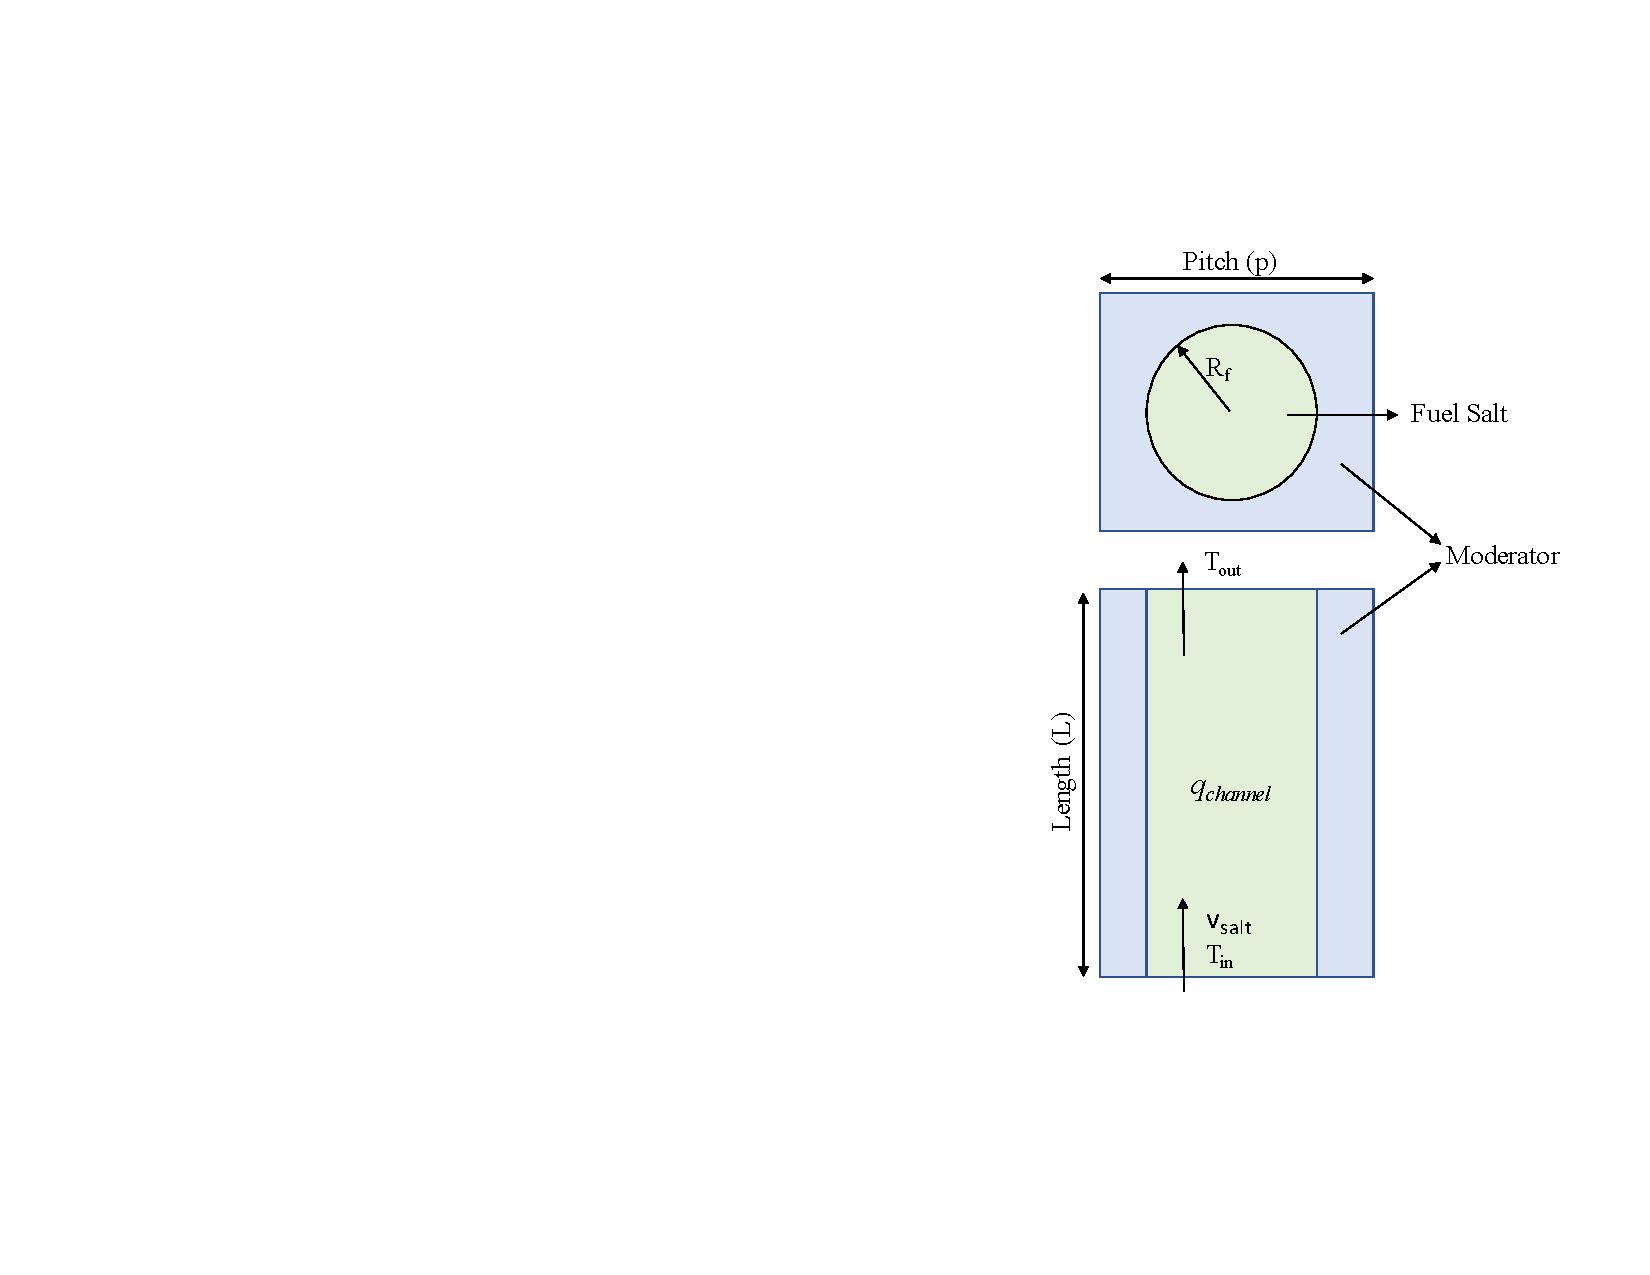
\includegraphics[trim=500 140 0 100, clip,
	scale=0.6]{images/single_channel.pdf}
	\caption{Single fuel channel representation}
	\label{fig:channel}
\end{figure}
%%%%%%%%%%%%%%%%%%%%%%%%%%%%%%%%%%%%%%%%
\begin{table}[ht!]
	\centering
	\caption{Feature parameters for database generation}
	\begin{tabular}{lllll}
		\hline
		\textbf{Variable} & \textbf{Distribution} & \textbf{Material types} &
		& \textbf{Steps} \\ \hline
		Fuel Type & Discrete   & U, U-Th, U-Pu & & 3 \\
		Salt Type & Discrete   & LiF-BeF$_2$, NaCl, & NaF-BeF$_2$  & 3 \\
		&  & \textbf{Lower value} &\textbf{Upper value} &  \\ 
		$f_{35}$  & Continuous  & 1 wt.\%   & 20 wt.\% & 10 \\
		$f_{U}$   & Continuous  & 10 wt.\%  & 90 wt.\% & 9 \\
		$p$       & Continuous  & 1 cm      & 16 cm & 10 \\
		$\xi$     & Continuous  & 0.274 & 10.46 & 10 \\
		$T_{ave}$ & Continuous  & 900 K     & 1200 K & 5 \\ \hline
	\end{tabular}
	\label{table:features}
\end{table}
%%%%%%%%%%%%%%%%%%%%%%%%%%%%%%%%%%%%%%%%

\subsubsection{Optimization Parameters}

We used the \gls{NSGAIII} \cite{deb2014, jain2014} from the pymoo tool
\cite{pymoo2020} as an optimizer with the \gls{SBX} and \gls{PM} operators. The
population size and number of generations were set to 150 and 5000,
respectively. Tournament selection, in which a set of chromosomes are selected
randomly and then the fittest chromosomes are selected for further operation,
was employed to select the fittest candidates from the current generation.

Several independent constraints imposed by the basic requisites of a \gls{MSR}
design were implemented to the solution objectives in accordance with the
references \cite{rykhlevskii2019, betzler2017, ashraf2019} in the following way:
$k_{\infty}$ is greater than 1.06 to make up for neutron leakage; $\varsigma$ is
higher than 0.6; and $\phi_{fast}$ per source neutron on graphite in which the
maximum value is calculated to be about 100 is less than 50.

In the optimization problem, the feature parameters were assigned as decision
variables while the performance metrics were assigned as solution objectives (or
objective functions). The $k_{\infty}$ and $\varsigma$ metrics were maximized
while the $\phi_{fast}$ was minimized.

\subsubsection{Neutronic Simulator}

We employed a Monte Carlo neutron transport tool, Serpent 2 (2.1.30)
\cite{Lep2014} to compute the performance metrics defined in design parameters
section. It uses ENDF/B-VII.0 \cite{chadwick2006} as the neutron cross-section
library along with S(${\alpha}$, ${\beta}$) thermal scattering libraries. In the
simulator, neutron population per cycle, passive cycle, and active cycle were
set to 2000, 50, and 100, respectively, to yield a computational standard error
of less than 100 pcm in the $k_{\infty}$. A two-group neutron energy structure
for the calculation of $\phi_{fast}$ on the moderator was used and lower and
upper energy boundaries for the fast region were set to 0.625 eV and 20 MeV,
respectively. The $k_{\infty}$, $\varsigma$, and $\phi_{fast}$ metrics were
directly extracted from the output file whereas ${\alpha_{total}}$ was
calculated by Eq. \protect\ref{Eq1}:
\begin{eqnarray}\label{Eq1}
\alpha_{total} = \dfrac{\partial\rho}{\partial T} \approx
\dfrac{\Delta\rho}{\Delta T}=\dfrac{\rho-\rho_b}{T-T_b}
\end{eqnarray}
where $\rho$ is the reactivity, $\rho_b$ is the reactivity at the base
temperature, $T$ is the temperature, and $T_b$ is the base temperature. However,
we purposefully avoided using $\partial \rho /\partial T$ in
estimating/predicting the feedback coefficient as ${\alpha_{total}}$ goes to
infinity when $T_{ave}$ is very close to the base temperature, resulting
problematic outputs. Instead, we used $\partial k$(mk) and converted to
${\alpha_{total}}$ at the end of the calculations. For the energy spectrum
classification of the reactor, the \gls{EALF}  value extracted from the output
file was used.

\subsubsection{Datasets}
In this work, a total training sample size of 285000 and a total test sample
size of 8000 were used.



	\section{Results}

\subsection{Preselection}

    For the estimators listed in Table~\ref{table:AImethods}, we presented performance score in Table~\ref{table:regression} for regression analysis and in Table~\ref{table:classification} for classification analysis. The results were obtained using the default hyperparameters. \gls{RF}, \gls{ET}, \gls{KN}, \gls{SVM}, and \gls{MLP} estimators predicted the performance metrics with significantly higher accuracy than the others. Even without hyperparameter optimization, \gls{R2} scores of these five estimators ranged from 90 to 98\% for regression and from 92 to 96\% for classification. This implies that the trained models by these estimators will have very low variance. The \gls{ET} regressor most accurately predicted the performance metrics while the \gls{SVM} classifier was superior to the others in classifying designs.

    In general, the linear methods (i.e., \gls{SGD}, \gls{R}, \gls{EN}, \gls{L}, \gls{LL}, \gls{P}, and \gls{Log}) yielded lower fit scores and higher errors with respect to the non-linear methods such as ensemble, \gls{SVM}, and \gls{ANN}. These results clearly imply that linear methods are not quite enough to design a nuclear reactor and thus in predicting its performance metrics. Like linear methods, the \gls{NB} classification methods such as \gls{GNB} and \gls{BNB} seem inappropriate due to the suboptimal performance scores. This is because these methods such as linear and \gls{NB} are not sufficient to fit the training dataset (leading to underfitting) into a linear function due to the higher degree interdependencies of our feature parameters. In addition to this, the \gls{RF}, \gls{DT}, \gls{B}, and \gls{AB} estimators, gave similar results, except for fit score values, as they use the same base estimator (\gls{DT}) in training. Likewise, the \gls{LP} classifier produced the same results with the \gls{SVM} classifier due to the use of the same kernel ($rbf$). In regression analysis, the \gls{ET} regressor has the lowest \gls{MAE} and \gls{MSE} scores while the \gls{R} regressor has the highest scores.

    As to the classification, the \gls{SVM} classifier has the lowest \gls{HL} and \gls{LRL} scores while the \gls{P} classifier has the highest scores. Briefly, any design can be classified with high precision ($>$ 95\%) and very few incorrectly predicted labels (false neagtive plus false positive: $<$ 5\%), leading to an opportunity for an accurate prediction of reactor design even without making any regression analysis.

    On the whole, five estimators (i.e., \gls{RF}, \gls{ET}, \gls{KN}, \gls{SVM}, and \gls{MLP}) that satisfy a score of more than 90\% in \gls{R2} and fit scores appear to be suitable for the subsequent stage of calculations. Among the selected estimators, the \gls{SVM} regressor interestingly shows the second-best performance right after the \gls{ET} regressor despite its worst fit score. In fact, as the scores of the best performing estimators are very close to each other, at this point, it is not easy to distinguish which estimator is the best. Therefore, in the following section, the current scores of these estimators are further improved by tuning their hyperparameters and investigating their learning curves.

%%%%%%%%%%%%%%%%%%%%%%%%%%%%%%%%%%%%%%%%
\begin{landscape}
	\begin{table}[ht!]
		\centering
		\caption{Performance scores of the studied regression methods}
		\begin{tabular}{l>{\columncolor[gray]{0.9}}l>{\columncolor[gray]{0.9}}
				l>{\columncolor[gray]{0.9}}l>{\columncolor[gray]{0.9}}
				l>{\columncolor[gray]{0.9}}lllllllllllllllllllllllllll}
			\hline
			& \textbf{\gls{RF}} & \textbf{\gls{ET}} & \textbf{\gls{KN}} &
			\textbf{\gls{SVM}} & \textbf{\gls{MLP}} & \textbf{\gls{DT}} & \textbf{GB} &
			\textbf{B} & \textbf{AB} & \textbf{SGD} & \textbf{R} & \textbf{EN} &
			\textbf{L} & \textbf{LL} \\
			\hline
			fit score & 1.00 & 1.00 	& 0.99  & 0.96 	& 0.99  & 1.00 & 0.97 & 1.00
			& 0.78	& 0.54 	& 0.73 	& 0.70 	& 0.69 	& 0.55 \\
			EVR  & 0.90 & 0.98 & 0.97 & 0.98 	& 0.95  & 0.90 &
			0.89 & 0.90 & 0.54	& 0.38 & 0.37 & 0.46 & 0.25 & 0.38 \\
			\gls{MAE} & 1.27 & 0.35	& 0.57  & 0.54 	& 0.87  & 1.28 &
			1.72 & 1.27 & 3.36 & 4.77 & 4.78 & 4.60 & 4.77 	& 4.77	\\
			\gls{MSE} & 7.60 & 0.62 & 1.61 & 1.45 & 2.97 & 7.71 & 12.99
			& 7.60 & 38.85 & 82.73	& 82.94	& 77.95	& 81.94	& 82.95	\\
			R$^2$ & 0.90 & 0.98 & 0.97 & 0.98 & 0.95  & 0.90 & 0.89 & 0.90 &
			0.00 & 0.23 & 0.22 & 0.35 & 0.07 & 0.23	\\
			\hline
		\end{tabular}
		\label{table:regression}
	\end{table}
	%%%%%%%%%%%%%%%%%%%%%%%%%%%%%%%%%%%%%%%%
	\begin{table}[ht!]
		\caption{Performance scores of the studied classification methods}
		\begin{tabular}{l>{\columncolor[gray]{0.9}}l>{\columncolor[gray]{0.9}}
				l>{\columncolor[gray]{0.9}}l>{\columncolor[gray]{0.9}}
				l>{\columncolor[gray]{0.9}}llllllllllllllllll}
			\hline
			& \textbf{\gls{RF}} & \textbf{\gls{ET}} & \textbf{\gls{KN}}	&
			\textbf{\gls{SVM}}   & \textbf{\gls{MLP}}& \textbf{\gls{DT}} &
			\textbf{\gls{B}} &
			\textbf{\gls{LP}} & \textbf{\gls{GB}}  & \textbf{\gls{AB}} &
			\textbf{\gls{SGD}}	& \textbf{\gls{R}} &
			\textbf{\gls{GNB}}  & \textbf{\gls{BNB}}& \textbf{\gls{P}}&
			\textbf{\gls{Log}}\\
			\hline
			fit score  	& 1.00 	& 1.00 	& 0.91 	& 0.90 	& 0.90 	& 1.00 	& 0.98 	& 0.90
			& 0.88 & 0.84 	& 0.61 	& 0.65 	& 0.64 	& 0.55 	& 0.45 	& 0.68\\
			\gls{AP} & 0.90 	& 0.93 	& 0.92 	& 0.95 	& 0.96 	& 0.90 	&
			0.90 	& 0.96 	& 0.91 & 0.90 	& 0.80 	& 0.69 	& 0.78 	& 0.52 	& 0.77 	& 0.81\\
			\gls{HL} & 0.05 	& 0.04 	& 0.04 	& 0.03 	& 0.04 	& 0.05 	&
			0.05 	& 0.04 	& 0.05 & 0.06 	& 0.17 	& 0.18 	& 0.13 	& 0.18 	& 0.22 	& 0.17\\
			\gls{LRAPS} & 0.94 	& 0.95 	& 0.95 	& 0.96 	& 0.96 	& 0.94 	& 0.94
			& 0.95 	& 0.94 & 0.93 	& 0.81 	& 0.81 	& 0.86 	& 0.82 	& 0.77 	& 0.82\\
			\gls{LRL} & 0.09 	& 0.07 	& 0.07 	& 0.06 	& 0.06 	& 0.09 	&
			0.09 	& 0.06 	& 0.08 & 0.09 	& 0.27 	& 0.28 	& 0.21 	& 0.27 	& 0.34 	& 0.27\\
			\gls{ROCAUC} & 0.92 	& 0.94 	& 0.94 	& 0.96 	& 0.95 	& 0.92 	&
			0.92 	&
			0.92 	& 0.93 & 0.93 	& 0.79 	& 0.70 	& 0.87 	& 0.60 	& 0.75 	& 0.77\\
			\hline
		\end{tabular}
		\label{table:classification}
	\end{table}
\end{landscape}
%%%%%%%%%%%%%%%%%%%%%%%%%%%%%%%%%%%%%%%%

\subsection{Hyperparameters optimization and learning curve}

    We applied two distinct methods to the estimators to improve their performance. The first method, expected to have an impact on the \gls{R2} scores, prediction errors, and thus cross-validation results, aims to find an optimal size for the training dataset. For this, Figure~\ref{fig:lc} demonstrates the estimator's learning curves for the (U-Th)F$_4$-NaF-BeF$_2$ fuel-salt pair from the viewpoint of \gls{R2} score in regression and multi-label classification accuracy in classification.

    At first look, the \gls{MLP} and \gls{SVM} predictive models do not require more data since the training and cross-validation scores converge together. On the contrary, the \gls{RF}, \gls{ET} and \gls{KN} models require more data as their training scores are much higher than their cross-validation scores.

    From all the learning curves, the \gls{RF}, \gls{ET}, \gls{MLP}, and \gls{SVM} models require a training size in the range of 32000 and 40000 in which the curves level off to a \gls{R2} score of 0.99 whereas the \gls{KN} model requires sample size more than 40000. A similar situation was observed in the classifiers' learning curves. As a result, we decided to use about forty thousand samples for each fuel-salt pair. In other words, for nine fuel-salt pairs, we generated around three hundred thousand samples in total. In the second method, we obtained optimal hyperparameters of the estimators tabulated in Table~\ref{table:hyper}. Parameters not listed in the table are at their default values and do not need optimization.

%%%%%%%%%%%%%%%%%%%%%%%%%%%%%%%%%%%%%%%
    \begin{figure}[ht!]
    	\begin{center}
    		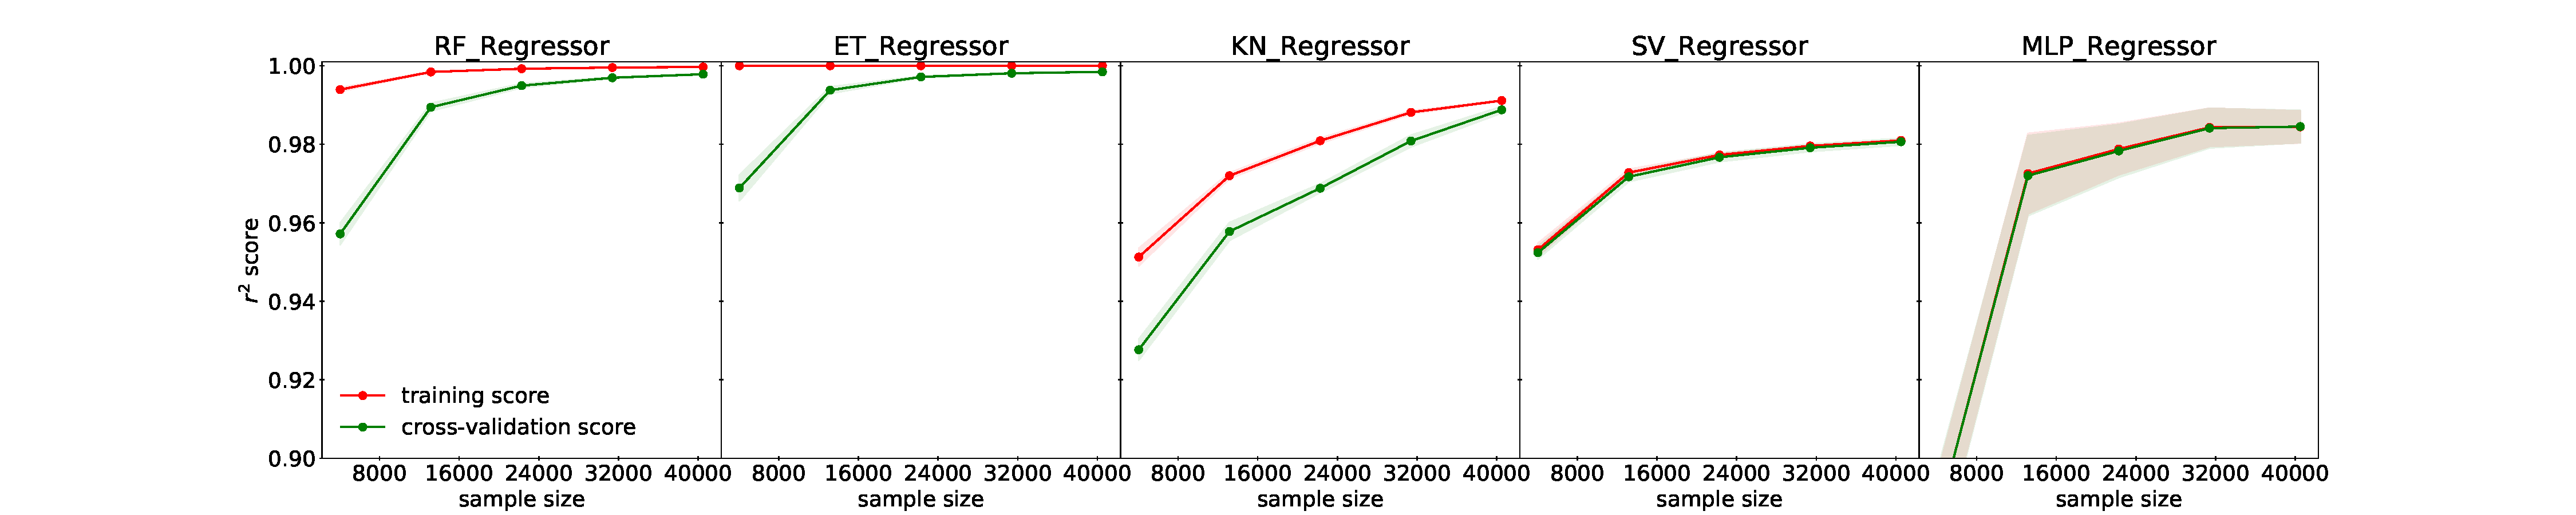
\includegraphics[trim=200 0 200 0, clip,
    		width=\textwidth]{images/regressors_learning_curves.pdf}

    		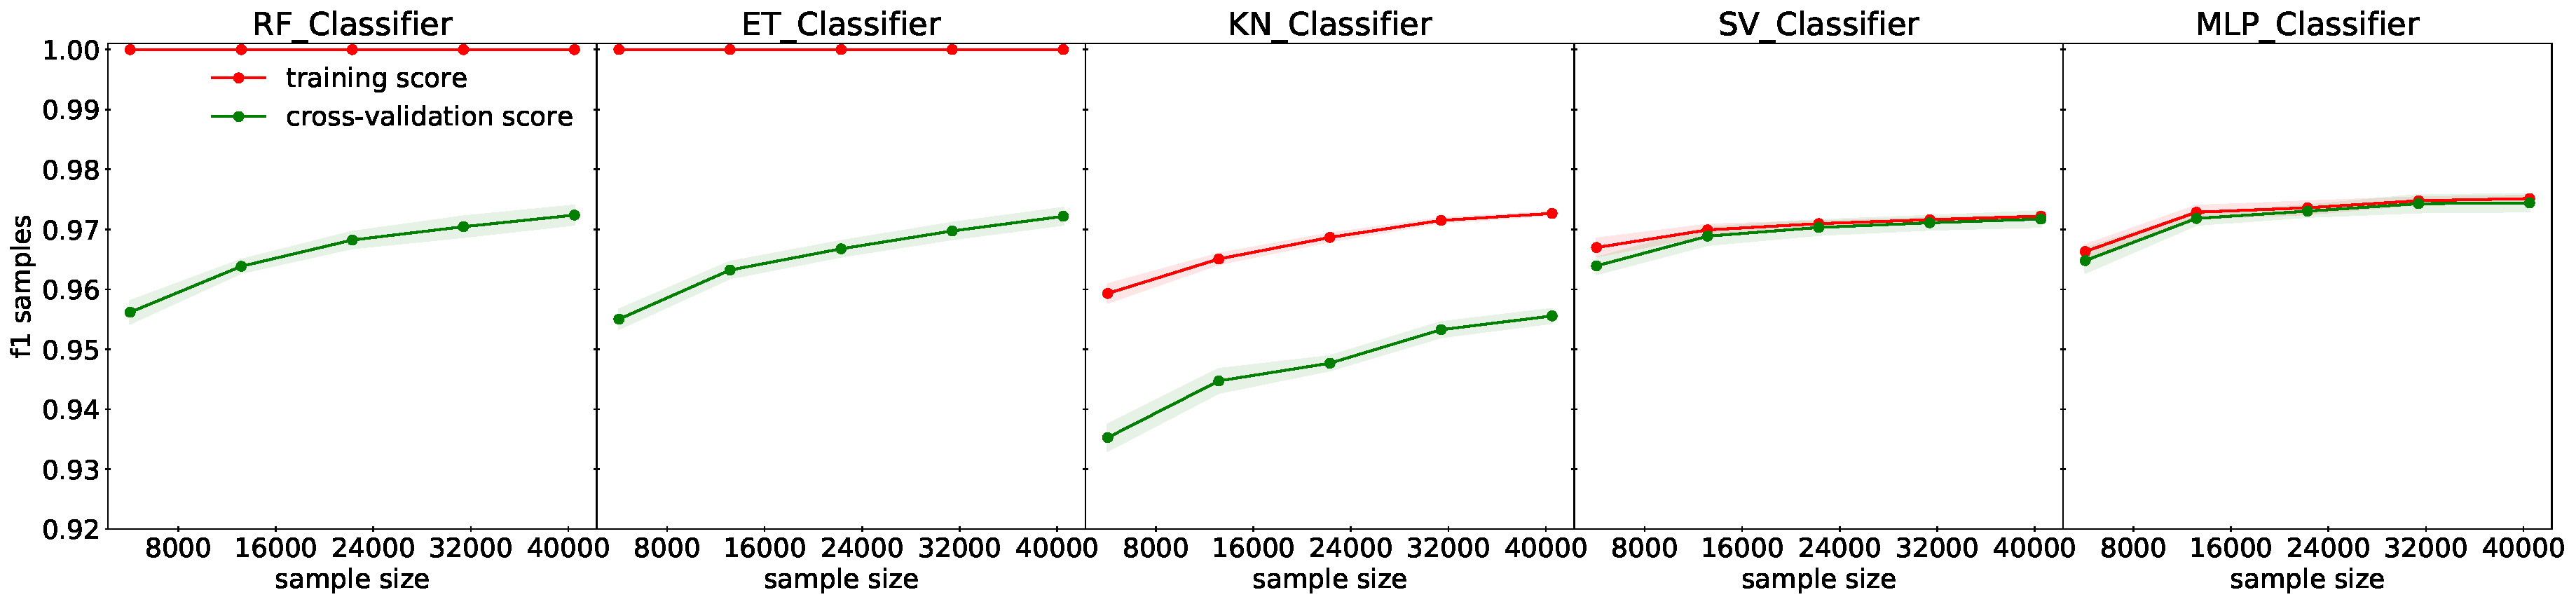
\includegraphics[width=\textwidth]{images/classifiers_learning_curves.pdf}
    	\end{center}
    	\caption{Learning curves of the selected estimators. Solid lines represent mean scores, while the shaded areas around lines represent the standard deviation of the mean due to error.}
    	\label{fig:lc}
    \end{figure}
%%%%%%%%%%%%%%%%%%%%%%%%%%%%%%%%%%%%%%%%
%%%%%%%%%%%%%%%%%%%%%%%%%%%%%%%%%%%%%%%%
\begin{table}[ht!]
	\centering
	\caption{Optimal hyperparameters of the selected estimators}
	\begin{tabular}{l p{0.8\linewidth}}
		\hline
		\textbf{Method} & \textbf{Parameters  (Regressor/Classifier)} \\
        \hline
		\gls{RF} & maximum features: None/None, number of trees: 400/400, minimum number of samples: 7/7                 \\
		\gls{ET} & maximum features: None/None, number of trees: 800/800, minimum number of samples: 1/7, quality criterion: -/gini    \\
		\gls{KN} & weight function: distance/distance, number of neighbors: 7/44, distance metric: manhattan/manhattan, leaf size: 136/200  \\
		\gls{SVM} & kernel type: rbf/poly, polynomial degree: -/3, kernel coefficient: auto/scale, epsilon: 0.1/-, regularization parameter: 3.4/1.2, stopping criterion: 1e-5 \\
		\gls{MLP} & activation function: relu/tanh, hidden layers: 1000/250, maximum iterations: 1e4/1e4, tol: 1e-5, solver: adam/sgd, learning rate: adaptive/constant       \\ \hline
	\end{tabular}
	\label{table:hyper}
\end{table}

\subsection{Final Estimators}

    After performing the hyperparameter optimization and learning curve assessment, we evaluated the final scores of the selected estimators and listed them in Table~\ref{table:finalreg} and ~\ref{table:finalclf}. At a glance, we saw that there is a slight enhancement in the performance scores of all regressors, except for the scores of the \gls{MLP} regressor that exhibits a strong hyperparameter dependency. However, the hyperparameter optimization did not improve the scores of the classifiers. With the optimized hyperparameters and data size in the training dataset, the \gls{ET}, \gls{SVM}, and \gls{MLP} regressors predicted performance metrics with a higher \gls{R2} and lower \gls{MAE} compared to their preselection scores.

    On the other hand, the \gls{SVM} and \gls{MLP} classifiers labeled the design attributes with the highest \gls{AP} and lowest \gls{LRL} scores relative to the other estimators. Nonetheless, the others are also suitable as all the scores are very close to each other. As the scores did not give us sufficient information about determining the right estimator for the next phase, we investigated cross-validation plots and multi-label confusion matrices on the basis of each performance metric (i.e., $k_{\infty}$, $\varsigma$, $\phi_{fast}$).

%%%%%%%%%%%%%%%%%%%%%%%%%%%%%%%%%%%%%%%%
    \begin{table}[ht!]
    	\centering
    	\caption{Final performance scores of the selected regressors}
    	\begin{tabular}{lllll>{\columncolor[gray]{0.9}}l}
    		\hline
    		& \textbf{\gls{RF}}  & \textbf{\gls{ET}}  & \textbf{\gls{KN}} &
    		\textbf{\gls{SVM}}   & \textbf{\gls{MLP}} \\
    		\hline
    		fit score  & 1.00 	& 1.00 & 1.00 & 0.97  & 1.00 \\
    		\gls{EVR} & 0.94 & 0.99 & 0.99 & 0.96 & 1.00 \\
    		\gls{MAE} & 1.07 & 0.28 & 0.41 & 0.37 & 0.23 \\
    		\gls{MSE} & 5.52 & 0.41 & 0.83 & 0.44 & 0.24 \\
    		R$^2$ & 0.94 & 0.99 & 0.98 & 0.96 & 1.00 \\
    		\hline
    	\end{tabular}
    	\label{table:finalreg}
    \end{table}
%%%%%%%%%%%%%%%%%%%%%%%%%%%%%%%%%%%%%%%%
    \begin{table}[ht!]
    	\centering
    	\caption{Final performance scores of the selected classifiers}
    	\begin{tabular}{lllll>{\columncolor[gray]{0.9}}l}
    		\hline
    		& \textbf{\gls{RF}} & \textbf{\gls{ET}}  & \textbf{\gls{KN}} &
    		\textbf{\gls{SVM}}  & \textbf{\gls{MLP}} \\
    		\hline
    		fit score  & 0.93 & 1.00 & 1.00  & 0.89 & 0.90 \\
    		\gls{AP} & 0.92 & 0.94 & 0.95  & 0.96 & 0.97  \\
    		\gls{HL} & 0.04 & 0.04 & 0.04  & 0.03 & 0.03  \\
    		\gls{LRAPS}  & 0.95 & 0.96 & 0.96  & 0.96 & 0.97 \\
    		\gls{LRL} & 0.07 & 0.06 & 0.06  & 0.05 & 0.05  \\
    		\gls{ROCAUC} & 0.94 & 0.95 & 0.96  & 0.95 & 0.96 \\
    		\hline
    	\end{tabular}
    	\label{table:finalclf}
    \end{table}
%%%%%%%%%%%%%%%%%%%%%%%%%%%%%%%%%%%%%%%%

\subsection{Cross-validation plot and confusion matrix}

    In this section, we compared the predicted test dataset with the actual test dataset. Figure~\ref{fig:cv} visualizes the predicted performance metrics against their actual values for the chosen estimators in terms of cross-validation plots. These plots show the estimator's prediction quality separately for each performance metric. Results indicated that the \gls{ET}, \gls{KN}, and \gls{MLP} estimators accurately predict performance metrics per the acceptance criterion (within $<$5\% relative error).

    According to these results, the \gls{ET} estimator is the best option to employ in the optimization phase. In comparison to the actual values, it correctly estimated the $k_{\infty}$ metric, slightly underestimated the $\varsigma$ metric, and predicted a few values of the $\phi_{fast}$ metric outside of the region. The \gls{KN} and \gls{MLP} estimators have good results comparable to the \gls{ET} and, therefore, be considered as alternative estimators for regression analysis.

    For classification analysis, we presented confusion matrices, normalized over the total test sample size, in Figure~\ref{fig:cm} to compare the predicted labels with the actual labels in terms of true/false positive and true/false negative scores. From the prediction capability standpoint, these estimators have very close scores in each label and predict all labels with high precision ($<$95\%). Related to the scores of the labels, the only label that causes the highest misclassification score by 10\% is the feedback coefficient. This mislabeling originates from the feedback coefficients very close to zero as they are not accurately estimated. Other labels were, however, correctly estimated with an error of less than 1\%. As a result, any of these classifiers can easily handle the classification of channel designs without causing a notable loss in labeling. In this context, as in the regression analysis, we decided to use the \gls{ET} classifier in the design optimization phase to estimate the labels of optimum designs.

    \begin{figure}[ht!]
     \begin{center}
            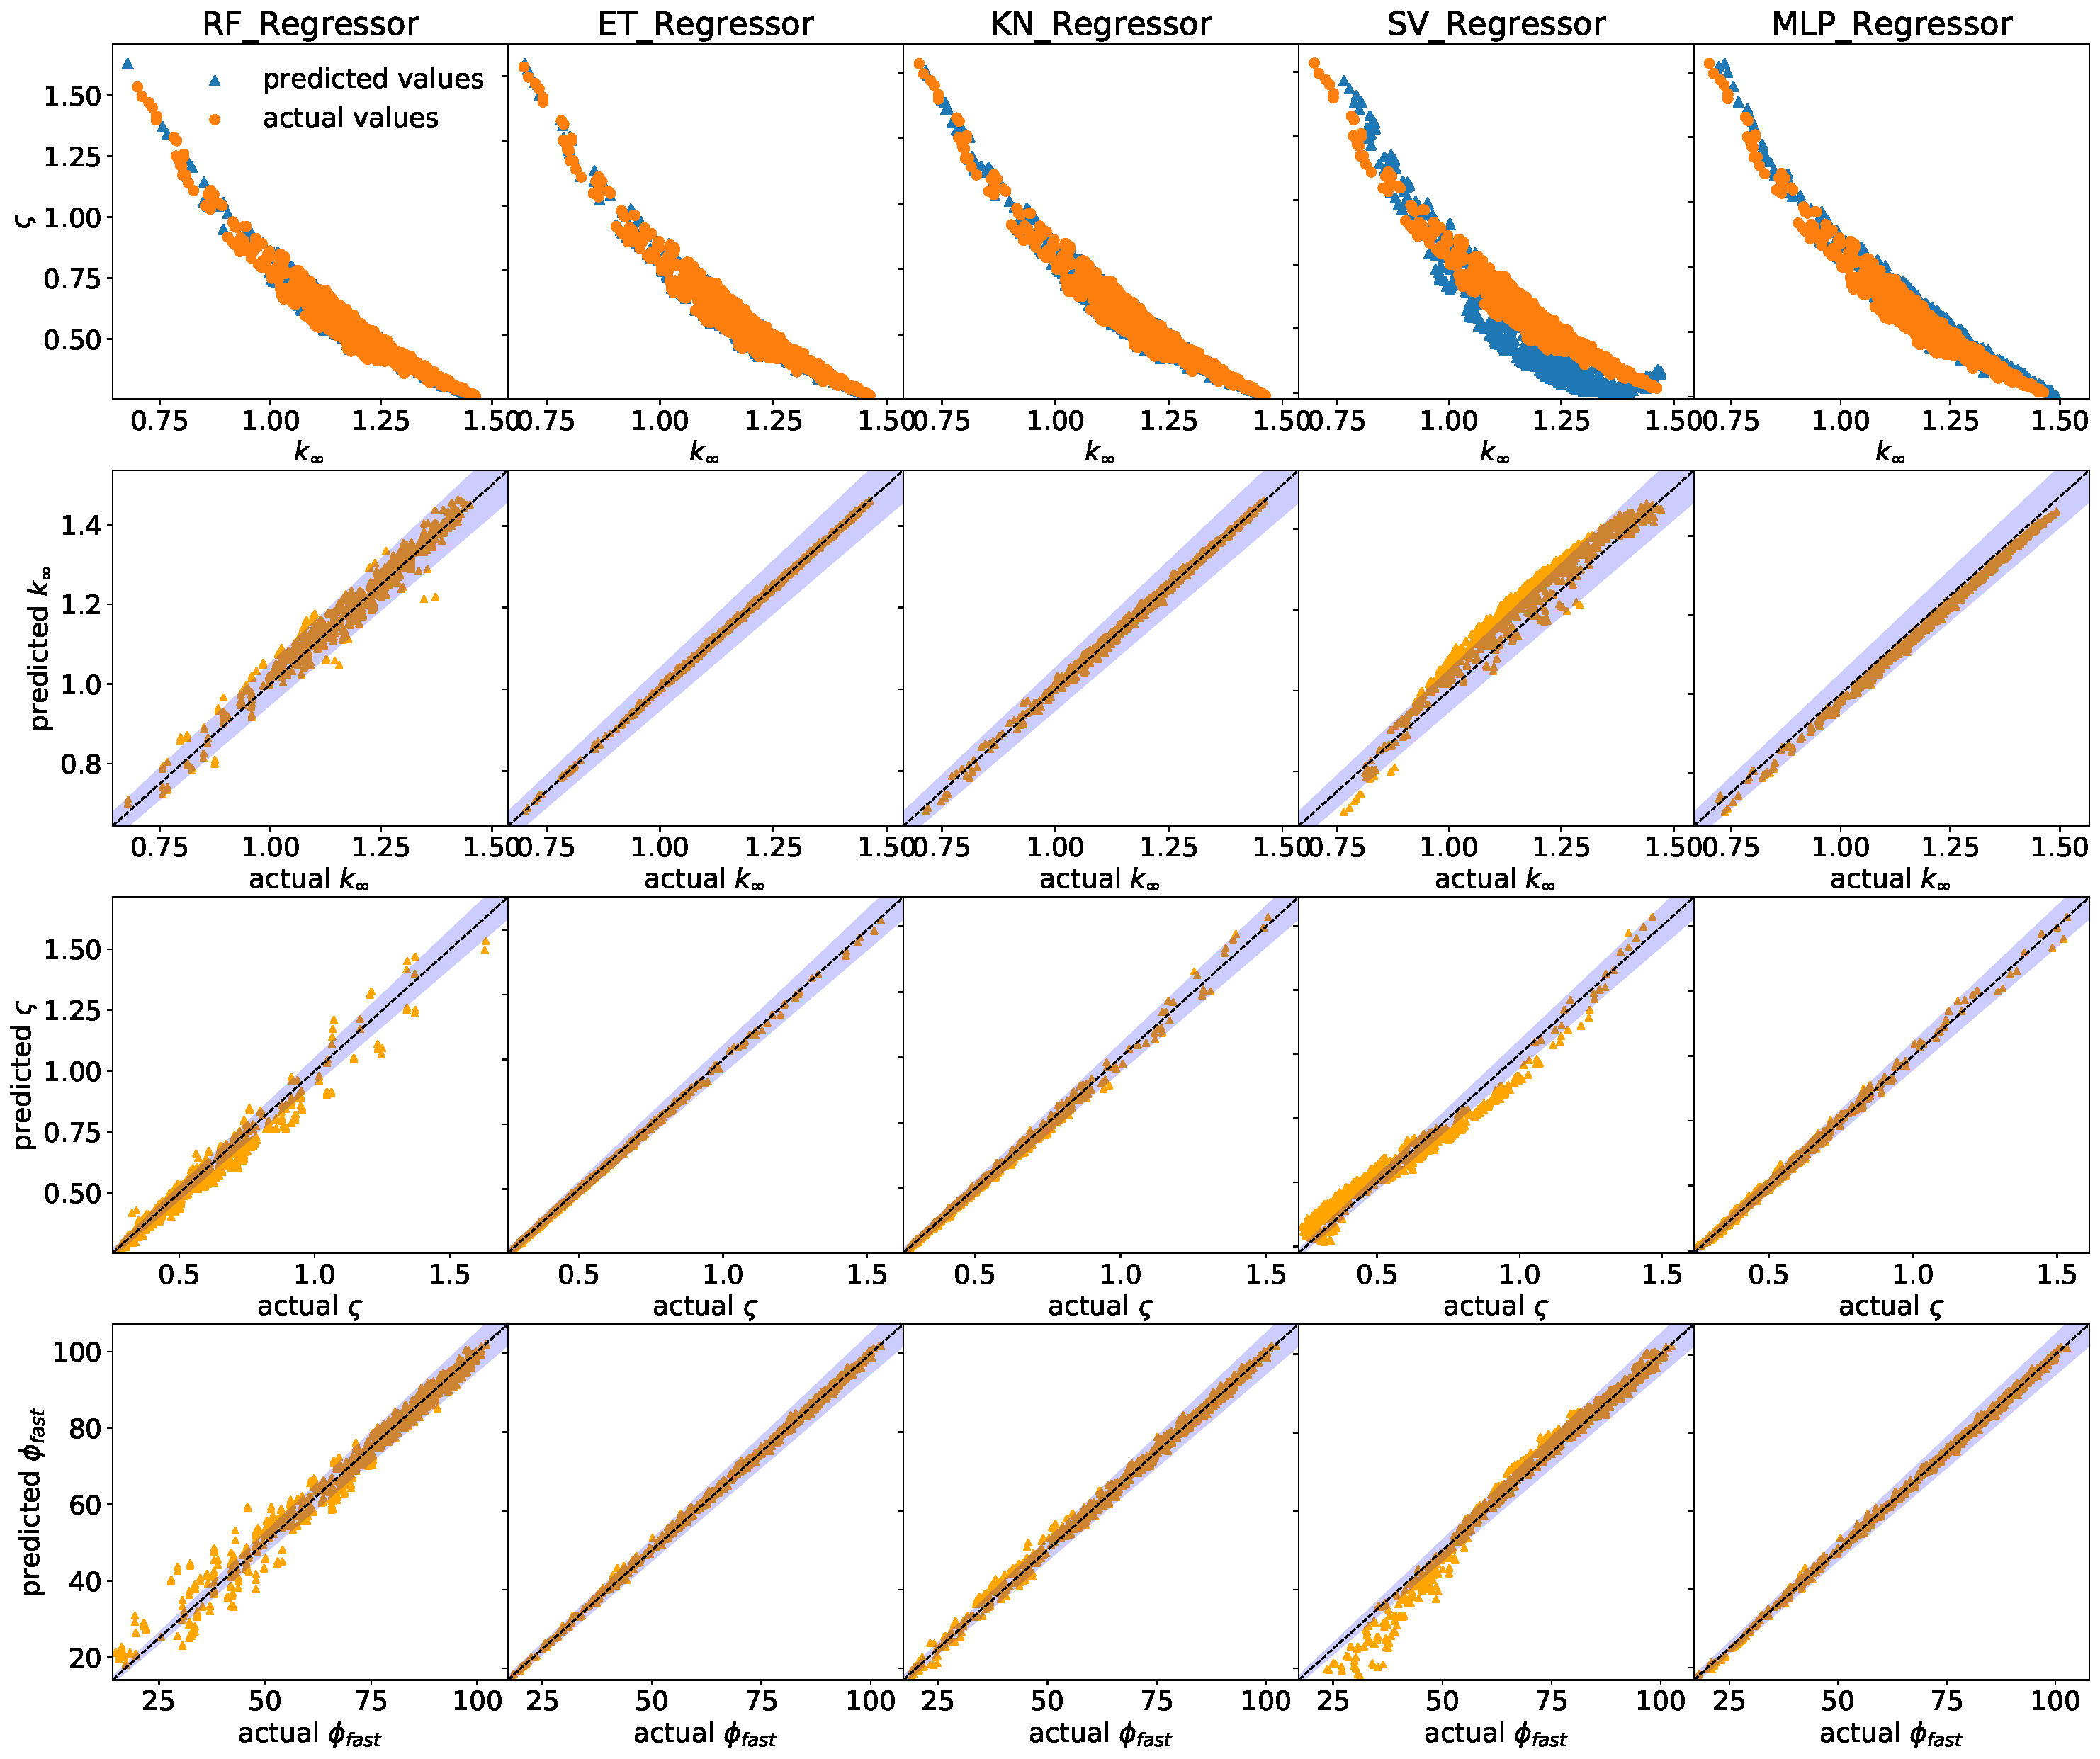
\includegraphics[width=\textwidth]{images/regression_cross_validation.pdf}
     \end{center}
        \caption{Cross-validation plots of the selected regressors, top to bottom:	(i)$k_{\infty}$ versus $\varsigma$ (ii) $k_{\infty}$ (iii) $\varsigma$ and	(iv) $\phi_{fast}$  }
        \label{fig:cv}
    \end{figure}
    \begin{figure}[htbp!]
     \begin{center}
            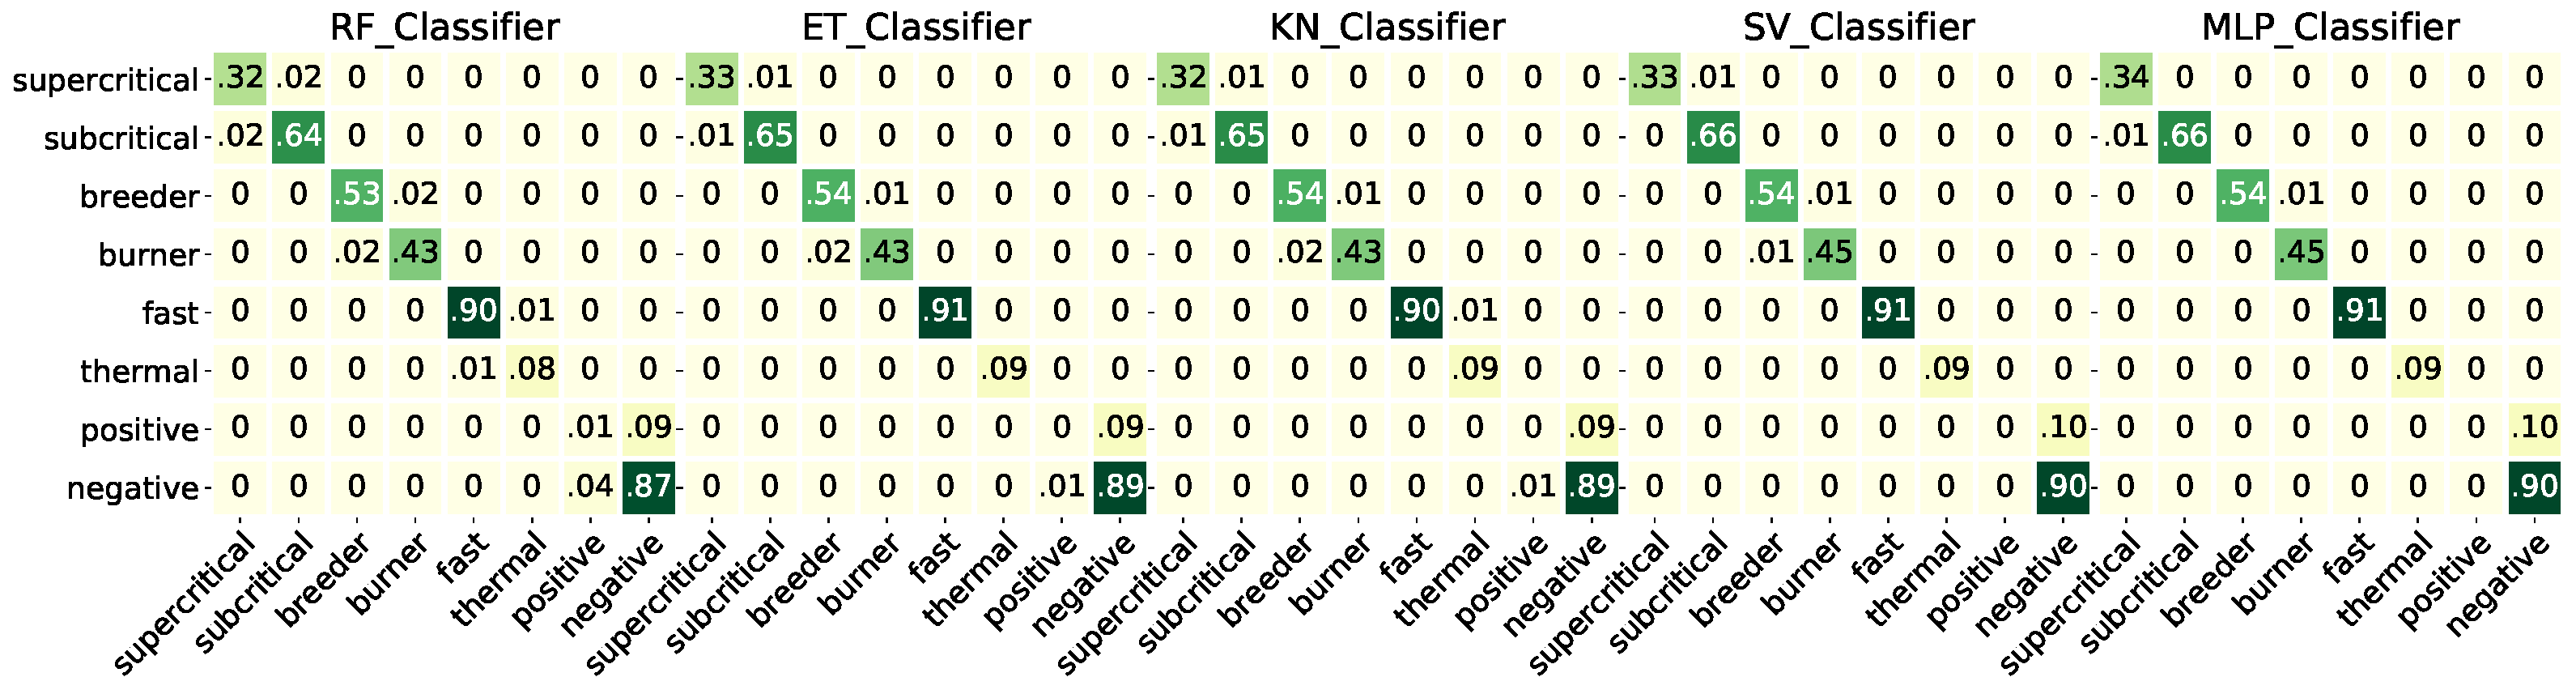
\includegraphics[width=\textwidth]{images/classification_confusion_matrix.pdf}
     \end{center}
        \caption{Normalized confusion matrices of the selected classifiers}
        \label{fig:cm}
    \end{figure}

\subsection{Optimum Designs}

    Based on the constraints applied to performance metrics, we found a set of optimum solutions for each fuel-salt pair. As an illustration, we presented the Pareto-front solutions for the (U-Th)F$_4$-NaF-BeF$_2$, which is very similar to the results of other fuel-salt pairs, in Figure~\ref{fig:pareto}. This figure includes (a) cross-validation plots for each performance metric, (b) the distribution of the Pareto-front solutions in 3-D performance metric space, and (c) the normalized confusion matrix. As seen from the subplot (a), the Pareto-optimal solutions (blue triangle) overlapped very well with the actual values (orange circles). The other subplots also confirm this situation by showing good distributions in the very proximity of the intersection line of each performance metric.

    The cross-validation subplots also indicated that all the predicted metrics totally stay within the 5\% relative error (shaded area) and very close to the intersection line. We found even better results for the $k_{\infty}$ metric with no more than 1\% relative error.

    As in the regression analysis results, the classification results of the optimal solutions in subplot (c) agreed very well with the actual labels. The only noteworthy complication is the misclassification of a tiny fraction of the feedback indicators. This mislabeling certainly arose from the prediction of the ${\alpha_{total}}$ values as discussed before and were estimated as positive instead of negative. In conformity with the constraints applied to performance metrics in the optimization phase, all the optimum designs we found are of characteristics of supercritical eigenvalue, fast spectrum, burner type, and negative feedback.

    Of the entire Pareto front solutions (around 650) which account for each combination of the fuel-salt pairs, only the nine best solutions are tabulated in Table~\ref{table:optimaldesigns}. We simply opted for the solutions that grant the highest breeding ratio ($\varsigma$) and the lowest fast flux ($\phi_{fast}$) at the $k_{\infty}$ = 1.06. The only exception for the multiplication factor criterion is for the NaCl salt in U-Pu fuel as there are no solutions with a multiplication factor less than 1.21 for this fuel-salt pair.

    As provided in the table, the suggested solutions can be grouped more easily by fuel type as the solutions show a certain relationship with the fuel type rather than the salt type. When the fuel types are compared to each other, U-Th fuels require the highest $^{235}$U content (18-20\%) due to the existence of the $^{232}$Th isotope which has an absorption cross-section approximately four times higher than $^{238}$U. U fuels reach their top performance when a moderate amount of $^{235}$U (14-15\%) is used. U-Pu fuels need the lowest amount of $^{235}$U (5\%) as not only does Pu in U-Pu already contain a certain fraction of fissile isotopes like $^{239}$Pu and $^{241}$Pu, but also Pu fissile isotopes emit greater average fission neutrons per absorption. Similarly, we noticed that U-Th fuels demand 13-14\% Th in U-Th while U-Pu fuels favor the highest grade of U content (90\%).

    A comprehensive look at the common properties of the optimal designs suggests that $T_{ave}$ should be in the range of 1100-1200 K and $\xi$ needs to be at its minimum value (0.274). Furthermore, as expected, Th necessitates higher fissile material than any other fuel types whereas the fissile material required by the U-Pu fuel is the lowest as the weapons-grade Pu comprises a gread deal of fissile isotopes by almost 50\% of its content. On the other hand, unlike the other feature parameters that display a direct characteristic relationship with the fuel type, there is no noticeable evidence to associate the channel-to-channel pitch length ($p$) with the fuel types. The $p$ parameter is, however, likely to vary with the salt type just as the NaCl salt calls for a constant pitch value of 1.0 cm in all fuel types.

    In summary, among the optimal designs, it appears that all the fuels mixed with the NaCl salt are the most promising designs. In particular, the F$_4$-PuF$_3$-NaCl fuel-salt yields the highest $\varsigma$ and $k_{\infty}$. The most unfavorable side of this fuel-salt is to have a lower ${\alpha_{total}}$ than other salt types but the coefficient is still quite sufficient compared to the exiting designs of \gls{MSR}s at the initial state with a total fuel-salt feedback coefficient of around -3.4 pcm/K \cite{rykhlevskii2019, robertson1971}. From the reactor safety point of view, the LiF-BeF$_2$ salt with the highest ${\alpha_{total}}$ is the most favorable.

    \begin{figure*}
    	\begin{center}
    		\begin{minipage}{.49\linewidth}
    			\begin{subfigure}[t]{1.0\linewidth}
    				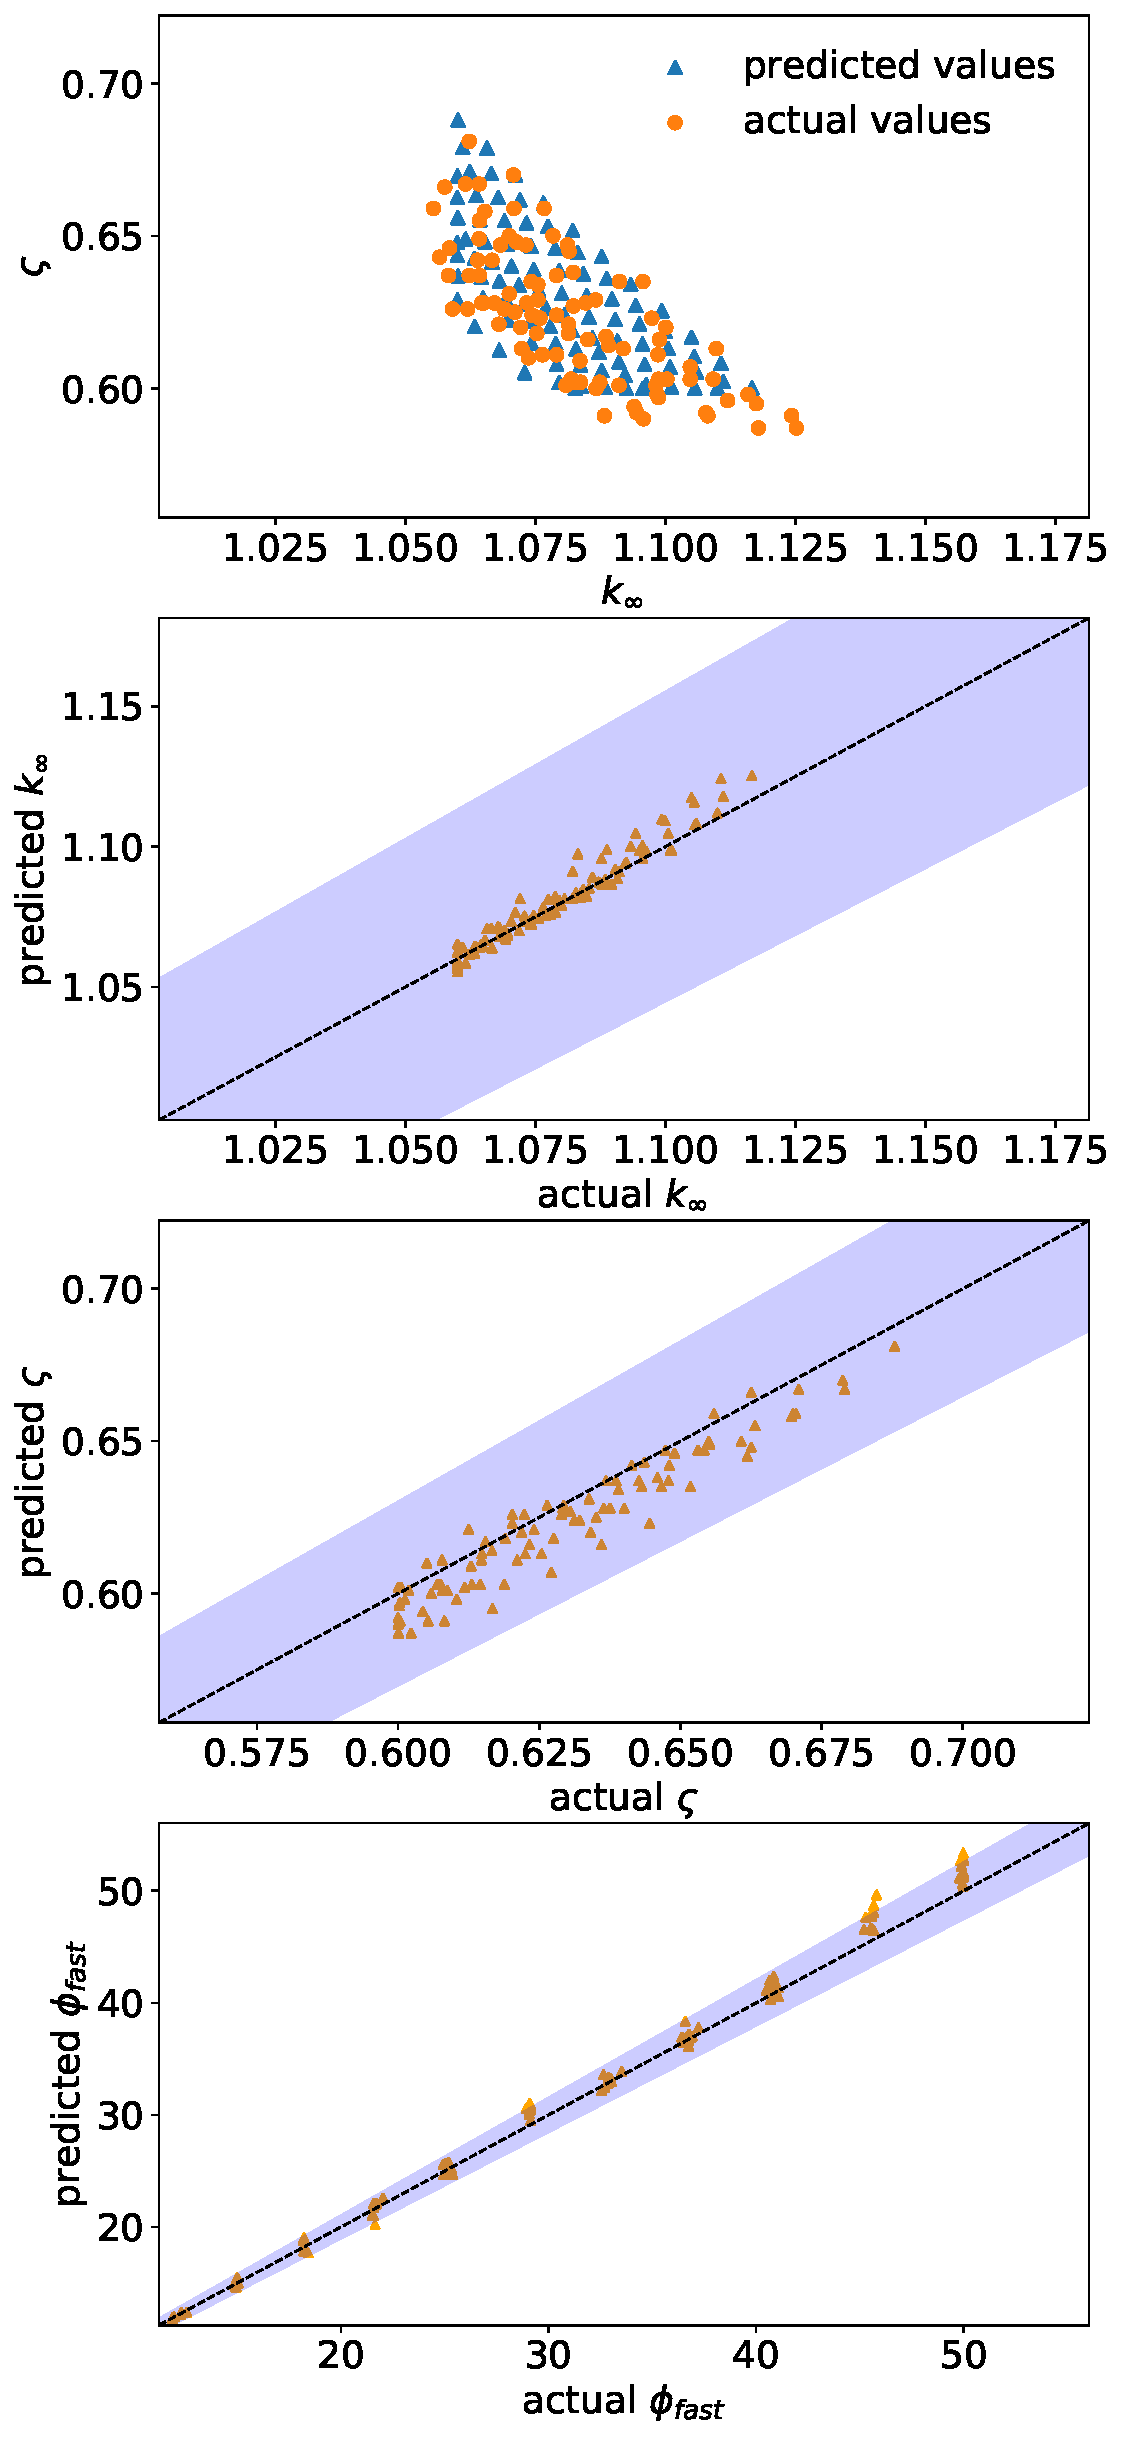
\includegraphics[width=\textwidth]{images/22_optimal_design_cross_validation.pdf}
    				\caption{}
    			\end{subfigure}
    		\end{minipage}
    		\begin{minipage}{.49\linewidth}
    			\begin{subfigure}[t]{1.0\linewidth}
    				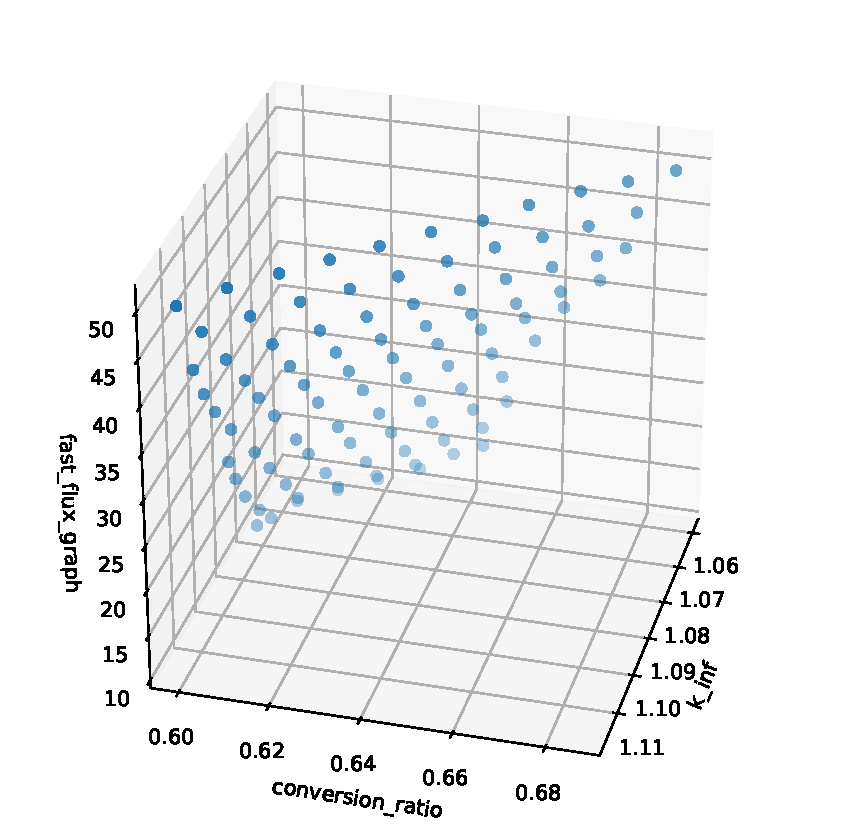
\includegraphics[width=\textwidth]{images/22_optimal_design_3d_solutions.pdf}
    				\caption{}
    			\end{subfigure} \\
    			\begin{subfigure}[b]{1.0\linewidth}
    				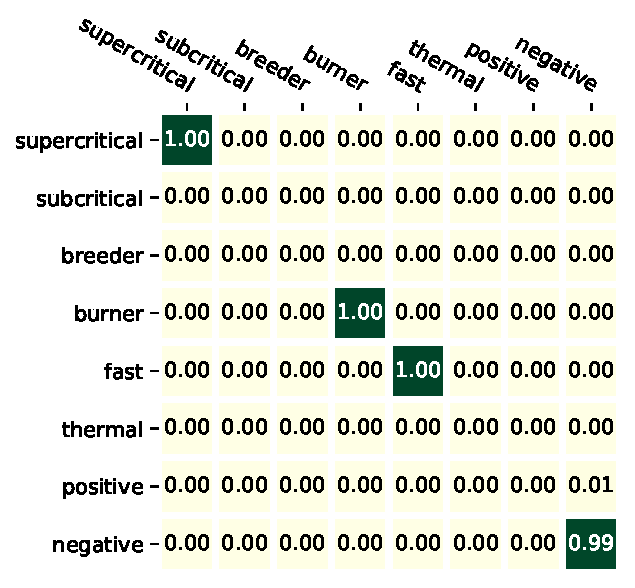
\includegraphics[width=\textwidth]{images/22_optimal_design_confusion_matrix.pdf}
    				\caption{}
    			\end{subfigure}
    		\end{minipage}
    	\end{center}
    	\caption{Optimum solutions for (U-Th)F$_4$-NaF-BeF$_2$: (a) cross-validation plots of performance metrics, (b) the distribution of the Pareto-front solutions in 3-D performance metric space, and (c) the normalized confusion matrix.}
    	\label{fig:pareto}
    \end{figure*}


%%%%%%%%%%%%%%%%%%%%%%%%%%%%%%%%%%%%%%%%
\begin{landscape}
	\begin{table}[ht!]
		\centering
		\caption{Optimal designs for each fuel-salt pair$^\star$}
		\begin{threeparttable}[t]
			\begin{tabular}{lllllllllll}
				\hline
				\textbf{Fuel Type} & \textbf{Salt Type}  & \textbf{$f_{35}$} &
				\textbf{$f_{U}$} & \textbf{$p$}	& \textbf{$T_{ave}$} & \textbf{$\xi$} &
				\textbf{$k_{\infty}$ \tnote{$\dagger$}}	& \textbf{$\varsigma$
					\tnote{$\ddagger$}}  & \textbf{$\phi_{fast}$ \tnote{$\perp$}} &
				\textbf{${\alpha_{total}}$ 	\tnote{$\wedge$}}  \\
				\hline

				U 	& LiF-BeF$_2$ 	& 14.47 & 100.0 & 86.7 & 1200 & 0.274 & 1.0600(+60) &
				0.661(-6) & 18.6(-0.5) 	& -3.9\\
				U 	& NaF-BeF$_2$ 	& 14.88 & 100.0 & 7.18 & 1125 & 0.274 & 1.0600(-120) &
				0.638(+6) & 19.0(-0.9) 	& -4.0\\
				U 	& NaCl 	& 14.28 & 100.0 & 1.00 & 1176 & 0.274 & 1.0604(-20) &
				0.692(0) & 12.6(0) 	& -3.0\\
				U-Th & LiF-BeF$_2$ 	& 19.10	& 86.7 & 5.50 & 1123 & 0.276 & 1.0601(-70) &
				0.665(-7) & 17.1(-0.2) 	& -4.3\\
				U-Th & NaF-BeF$_2$ 	& 20.00 & 86.8 & 5.98 & 1125 & 0.275 & 1.0600(+30) &
				0.643(-11) & 16.0(-0.2) & -2.8\\
				U-Th 	& NaCl 	& 18.48	& 86.2 	& 1.00 	& 1199 & 0.274 & 1.0600(+140) 	&
				0.696(-1) & 14.4(0)	& -2.8\\
				U-Pu & LiF-BeF$_2$ 	& 5.00 	& 90.0 	& 4.40 	& 1198 & 0.274 & 1.0600(-20) &
				0.732(+3) & 16.0(0.2) & -4.5\\
				U-Pu	& NaF-BeF$_2$ 	& 5.00 	& 89.3 & 4.37 & 1125 & 0.275 & 1.0600(+460) &
				0.723(+15) & 13.6(0.3) 	& -3.3\\
				U-Pu	& NaCl & 5.00 & 90.0 & 1.00 & 1193 	& 0.274 & 1.2192(+10) &
				0.753(+1) & 13.0(0)	& -3.4\\
				\hline
			\end{tabular}
            \rule{0in}{1.2em}$^\star$\scriptsize Performance metrics given in the table are the predicted values. The values inside the brackets are the actual values in terms of difference from the predicted values.

			\rule{0in}{1.2em}$^\dagger$\scriptsize The computational error of the infinite multiplication factor is $\pm$0.0009. The values within the brackets are in the units of pcm.

			\rule{0in}{1.2em}$^\ddagger$\scriptsize The computational error of the conversion ratio is $\pm$0.005. The values within the brackets are in the units of milli.

			\rule{0in}{1.2em}$^\perp$\scriptsize The computational error of the fast flux is $\pm$0.007.

			\rule{0in}{1.2em}$^\wedge$\scriptsize The propagated computational error of the feedback coefficient of reactivity is $\pm$0.4.

		\end{threeparttable}
		\label{table:optimaldesigns}
	\end{table}

\end{landscape}

%%%%%%%%%%%%%%%%%%%%%%%%%%%%%%%%%%%%%%%%

	\section{Conclusion} This study explored the promise of artificial
intelligence/machine learning techniques to identify optimal designs for a
single channel of a \gls{MSR}. We first created a reactor database to train and
test \gls{ML} methods and searched for the best performing estimator among those
\gls{ML} methods by evaluating their scores, cross-validation plots, and
confusion matrices. After deciding on the estimator, we used the genetic
algorithm technique (\gls{NSGAIII}) coupled to the selected estimator (\gls{ET})
to seek for the optimum single channel designs. We found a set of optimum
solutions for each fuel-salt pair considering several design constraints on the
performance metrics (i.e., fuel type, salt type, $^{235}$U fraction in U, U
fraction in heavy metal, channel-to-channel pitch length, moderator-to-salt
(volume) ratio, and average fuel-salt temperature). We accurately classified and
predicted design performance metrics. Major findings throughout this study and
general remarks on the results follow:

\paragraph{ As a result of the assessment of the scores of the estimators,
	\gls{RF}, \gls{ET}, \gls{KN}, \gls{MLP}, and \gls{SV} were chosen as the best
	candidate estimators for the design optimization phase} Estimators of ensemble,
support vector, \gls{NN}, and decision tree methods performed well, while the
linear methods (L, R, SGD etc.) performed poorly as compared to the non-linear
methods (\gls{DT}, GB, and \gls{RF} etc.). \paragraph{We evaluated a total
	optimum sample size of 300,000 for sufficiently accurate results} The learning
curves of the selected estimators suggested an optimum sample size in the
dataset of at least 12,000 for each fuel-salt pair. \paragraph{The \gls{ET}
	estimator was selected as the best estimator} The cross-validation plots and
confusion matrices of the candidate estimators shed light on the best estimator
for the design optimization phase by pinpointing the individual performance
metric. All the performance metrics were predicted with less than 5\% error and
classified with less than 1\% error except for the feedback label which has an
error of 10\%.  We also understood that the \gls{MLP} handles performance
metrics as good as \gls{ET}, but with considerably higher computational
run-time. \paragraph{We estimated all the performance metrics of the optimum
	designs within a prediction error of at most 5\% in comparison to their actual
	values} A comprehensive overview of the common properties of the optimal designs
implied a particular enrichment level and U content associated with fuel type
but not salt type, $T_{ave}$ higher than 1100 K, and a moderator-to-salt ratio
of 0.274. The relation of the channel-to-channel pitch length, $p$, with either
fuel type or salt type was not as clear as the other feature variables.
\paragraph{All the optimum designs were accurately labeled as supercritical
	reactor, burner type, fast spectrum, and negative flag in feedback coefficient}
As indicated by confusion matrices, only a few, most of which belong to the
feedback coefficient, were mislabeled.

\paragraph{Based on the constraints in this study, the optimal fuel-salt option
	was a combination of U-Pu fuel and NaCl salt} It achieved the longest graphite
lifetime (i.e., the lowest $\phi_{fast}$), the highest $\varsigma$, and a
sufficient negative ${\alpha_{total}}$.

In addition to the above numerical findings, the most important success of this
study is the integration of the \gls{ML}-enabled technique into the reactor core
design process. Another important success achieved by this proposed method is
the examination of the optimal designs in a very short time (within minutes),
regardless of the value and number of performance metrics or feature parameters,
once a reactor database is generated. Without using any reactor physics code,
this method makes available evaluating the performance metrics of any design
with very high accuracy by using a training dataset specific to the feature
parameters of interest to be loaded from a reactor database generated initially.
Due to the very fast computing speed and high accuracy in estimating performance
metrics, we recommend using this method for neutronic calculations (also for
thermal-hydraulics) in nuclear engineering along with nuclear computer codes
such as deterministic and Monte Carlo that require a significant user expertise.

In addition to these achievements, we encountered various difficulties that have
an direct and indirect impact on the outcomes of this study throughout the work.
First, we understood that the number of performance metrics, sample size, and
assigning different estimators (composite estimators) to an individual
performance metric significantly affect the errors of performance metrics. For
instance, the larger the sample size in the training dataset, the higher the fit
scores, thus better fitting results. Second, there were several known drawbacks
to getting better estimators' scores: one was the hyper-parameter dependency
influencing the scores of the estimators and the other one was the dependency on
the quality of training datasets containing out-of-interest values (outliers),
such as very low $k_{\infty}$ and very high $\varsigma$. Although the effects of
hyper-parameters are limited, outliers have a profound effect on the fit scores,
therefore on the predicted performance metrics and optimal designs.

We also figured out throughout this study that the primary difficulty with
regard to the applicability of \gls{ML} methods for reactor design is to
generate a reactor database which consumes the entire computer's resources,
requires a powerful supercomputer, and takes a long time. In fact, this is not a
critical issue for the applicability of the proposed method since the database
generation is quite easy process in comparison to other tasks and it is enough
to do it once at the very beginning of the study. Third, it is likely to find
different solutions when the population size and number of generations are
further increased, or a different optimization method, such as brute force which
scans the entire grid space for a global optimum solution, is used. But, we
anticipate that all the solutions to be obtained using different parameters
would be close to the global optima presented in this work as we already
verified our solutions with different optimizers and their varying
hyper-parameters. The only concern with the optimization process is the defined
constraints on performance metrics as an optimizer directs offspring according
to these constraints.

In our follow-up studies, we will take the following steps to do away with some
of the assumptions and simplifications we have made in this research, to
complement the shortcomings in the study and to further improve the existing
method. Initially, we have a plan to use the suggested method for a full-core
(or small scale or assembly) \gls{MSR} design in the second phase of the ongoing
study. Different from the single channel design, designing a full reactor core
will bring several additional variables (e.g., number of fuel channels, reactor
diameter) to the existing feature parameters and a few additional performance
metrics (e.g., power peaking factor) to the existing performance metrics. The
rest is expected to follow the method suggested in this study. Concurrently, we
will replace the grid-based search technique used in generating the reactor
database by a more sophisticated sampling strategy (e.g., adaptive, stratified
and hybrid), which would help reduce the number of datasets, by focusing only on
a particular domain. This is because, despite being the simplest and capable of
evaluating all the possible scenarios among the different parameters of feature
space, the technique is computationally expensive and consumes computing
resources by a considerable amount. On the other hand, in order to simplify the
optimization problem and make a significant gain in the simulation run-time, we
had deliberately disregarded the thermal-hydraulics effects such as delayed
precursor movement, temperature distribution along the channel, and reactivity
feedback on the neutronic calculations. Related to this, we will integrate the
Moltres MOOSE application that solves the thermal-hydraulics and neutronics
equations for liquid-fueled \gls{MSR}s with the Plankton python tool having been
developed in this work and increase the accuracy of neutronic calculations.

To sum up, this study has explored an approach to designing a nuclear reactor
core from scratch by incorporating the \gls{AI}/\gls{ML} techniques into single
channel analysis. The main focus of this study was to compare the prediction
accuracy of different \gls{ML} methods with each other and to decide the best
estimator suitable for single channel analysis. The research will make a
significant contribution to the further advancement of optimization studies by
eliminating the deficiencies of existing methods in reaching ideal designs such
as the tournament approach of the optimizers, convergence criteria, strict
constraints on performance metrics and concerns about computer resource
utilization. The results of this study could benefit researchers who are
interested in a multi-purpose reactor design which provides more flexibility for
in-core fuel management, improved neutron economy for fuel utilization, more
safety margin against core melt-down, prolonged reactor life-time, and less
spent nuclear fuel.

	\section{Acknowledgments}
This research is part of the Blue Waters sustained-petascale computing project,
which is supported by the National Science Foundation (awards OCI-0725070 and
ACI-1238993) and the state of Illinois. Blue Waters is a joint effort of the
University of Illinois at Urbana-Champaign and its National Center for
Supercomputing Applications.
The authors would also like to acknowledge financial support from the
Scientific and Technological Research Council of Turkey (TUBITAK) BIDEB-2219
Postdoctoral Research Program.
Prof. Huff is supported by the Nuclear Regulatory Commission Faculty
Development Program, the Blue Waters sustained-petascale computing project
supported by the National Science Foundation (awards OCI-0725070 and
ACI-1238993) and the state of Illinois, the NNSA Office of Defense Nuclear
Nonproliferation R$\&$D through the Consortium for Verification Technologies
and the Consortium for Nonproliferation Enabling Capabilities (awards
DE-NA0002576 and DE-NA0002534), the DOE ARPA-E MEITNER Program (award
DE-AR0000983), and the International Institute for Carbon Neutral Energy
Research (WPI-I2CNER), sponsored by the Japanese Ministry of Education,
Culture, Sports, Science and Technology.

	
	\bibliography{bibliography}
	
\end{document}
